%%%%%%%%%%%%%%%%%%%%%%%%
%% Sample use of the infthesis class to prepare a thesis. This can be used as
%% a template to produce your own thesis.
%%
%% The title, abstract and so on are taken from Martin Reddy's csthesis class
%% documentation.
%%
%% MEF, October 2002
%%%%%%%%%%%%%%%%%%%%%%%%

%%%%
%% Load the class. Put any options that you want here (see the documentation
%% for the list of options). The following are samples for each type of
%% thesis:
%%
%% Note: you can also specify any of the following options:
%%  logo: put a University of Edinburgh logo onto the title page
%%  frontabs: put the abstract onto the title page
%%  deptreport: produce a title page that fits into a Computer Science
%%      departmental cover [not sure if this actually works]
%%  singlespacing, fullspacing, doublespacing: choose line spacing
%%  oneside, twoside: specify a one-sided or two-sided thesis
%%  10pt, 11pt, 12pt: choose a font size
%%  centrechapter, leftchapter, rightchapter: alignment of chapter headings
%%  sansheadings, normalheadings: headings and captions in sans-serif
%%      (default) or in the same font as the rest of the thesis
%%  [no]listsintoc: put list of figures/tables in table of contents (default:
%%      not)
%%  romanprepages, plainprepages: number the preliminary pages with Roman
%%      numerals (default) or consecutively with the rest of the thesis
%%  parskip: don't indent paragraphs, put a blank line between instead
%%  abbrevs: define a list of useful abbreviations (see documentation)
%%  draft: produce a single-spaced, double-sided thesis with narrow margins
%%
%% For a PhD thesis -- you must also specify a research institute:
\documentclass[msc,frontabs,logo,twoside,deptreport]{infthesis}


%% For an MPhil thesis -- also needs an institute
% \documentclass[mphil,ianc]{infthesis}

%% MSc by Research, which also needs an institute
% \documentclass[mscres,irr]{infthesis}

%% Taught MSc -- specify a particular degree instead. If none is specified,
%% "MSc in Informatics" is used.
% \documentclass[msc,cogsci]{infthesis}
% \documentclass[msc]{infthesis}  % for the MSc in Informatics

%% Master of Informatics (5 year degree)
% \documentclass[minf]{infthesis}

%% Undergraduate project -- specify the degree course and project type
%% separately
% \documentclass[bsc]{infthesis}
% \course{Artificial Intelligence and Psychology}
% \project{Fourth Year Project Report}

%% Put any \usepackage commands you want to use right here; the following is
%% an example:
\usepackage[toc,page]{appendix}
\usepackage{natbib}
\usepackage{multicol}
\usepackage{float}
\usepackage{graphicx}
\usepackage{hyperref}
\usepackage{url}
\usepackage{wrapfig}
\usepackage{lscape}
\usepackage{rotating}
\usepackage{epstopdf}
\usepackage{tabu}
\usepackage{epigraph}
\usepackage{longtable}
\usepackage{listings}
\usepackage{xcolor}
\usepackage{array}
\usepackage{lipsum} % for dummy text
\usepackage{enumitem}
\setlist{nosep}
\usepackage[english, status=draft]{fixme}
\usepackage[colorinlistoftodos]{todonotes}
\fxusetheme{color}
\usepackage[font=small,labelfont=bf,justification=centering]{caption}
\captionsetup{justification   = raggedright,
              singlelinecheck = false}
\usepackage{multirow}
\graphicspath{ {resources/picture/},{resources/FE/},{resources/evaluation/}}


\colorlet{punct}{red!60!black}
\definecolor{background}{HTML}{EEEEEE}
\definecolor{delim}{RGB}{20,105,176}
\colorlet{numb}{magenta!60!black}

\lstdefinelanguage{json}{
    basicstyle=\normalfont\ttfamily,
    numbers=left,
    numberstyle=\scriptsize,
    stepnumber=1,
    numbersep=8pt,
    showstringspaces=false,
    breaklines=true,
    frame=lines,
    backgroundcolor=\color{background},
    literate=
     *{0}{{{\color{numb}0}}}{1}
      {1}{{{\color{numb}1}}}{1}
      {2}{{{\color{numb}2}}}{1}
      {3}{{{\color{numb}3}}}{1}
      {4}{{{\color{numb}4}}}{1}
      {5}{{{\color{numb}5}}}{1}
      {6}{{{\color{numb}6}}}{1}
      {7}{{{\color{numb}7}}}{1}
      {8}{{{\color{numb}8}}}{1}
      {9}{{{\color{numb}9}}}{1}
      {:}{{{\color{punct}{:}}}}{1}
      {,}{{{\color{punct}{,}}}}{1}
      {\{}{{{\color{delim}{\{}}}}{1}
      {\}}{{{\color{delim}{\}}}}}{1}
      {[}{{{\color{delim}{[}}}}{1}
      {]}{{{\color{delim}{]}}}}{1},
}


%% Information about the title, etc.
\title{What was I meant to do again (Exploration of event boundary on the failure of prospective memory)}
\author{Aldy Syahdeini}

%% If the year of submission is not the current year, uncomment this line and
%% specify it here:
% \submityear{1785}

%% Optionally, specify the graduation month and year:
% \graduationdate{February 1786}

%% Specify the abstract here.
\abstract{%

Prospective memory is remembering to carry out planned action in the future wihtout
instructed to do so.
The prospective memory failure is the common phenomena in everyday life.
The effect of prospective memory failure can be trivial but can also be critical. The topic and the experiment
of this research is based on the experiment conducted by Carlson and his team.
Different component of prospective memory and what aspect influence people to experience the failure was investigated.

An application to conduct a prospective memory experiment is developed.
The application is made flexible so different type of experiment properties can be implemented in the experiment.
The experiment on the failure of prospective memory is also conducted. Data were derived from 18 participants who underwent 3 experimental studies.
The experiment shows that the prospective memory error happens when people use a smartphone.
The amount of intentions is a crucial component of prospective memory
and the mental and physical transition influence of prospective memory error.
}

%% Now we start with the actual document.
\begin{document}

%% First, the preliminary pages
\begin{preliminary}

%% This creates the title page
\maketitle

%% Acknowledgements
\begin{acknowledgements}
Many thanks to my supervisor Dr. Maria wolters who put her believe on me, and her guidance
on the thesis.
Special thanks to Catherine crompton for useful discussions, hints, and
advice.
thanks to Prof. Richard Alan Carlson who give me an further understanding about this topic.
Big thanks to all my family and friends who always support me when I am working on my thesis.
Lastly, thank you for all the participants who participate on this experiment.


\end{acknowledgements}

%% Next we need to have the declaration.
\standarddeclaration

%% Finally, a dedication (this is optional -- uncomment the following line if
%% you want one).
% \dedication{To my mummy.}

%% Create the table of contents
\tableofcontents

%% If you want a list of figures or tables, uncomment the appropriate line(s)
% \listoffigures
% \listoftables

\end{preliminary}

%%%%%%%%
%% Include your chapter files here. See the sample chapter file for the basic
%% format.

\clearpage
\vspace*{\fill}
\begin{center}
\begin{minipage}{.6\textwidth}
  \textit{Don't worry, at the end it's gonna be good}

  - Dr. Maria wolters
\end{minipage}
\end{center}
\vfill % equivalent to \vspace{\fill}
\clearpage


\chapter{Introduction}
 \epigraph{Every moment of consciousness is a precious and fragile gift.}{\textit{Steven Pinker}}

\section{Prospective Memory error}


Have you experienced when you wake up from your bed in the morning, put your glasses on and
go to the kitchen to get a glass of milk. But when you are in the kitchen, you forget what
you intended to do. This phenomenon is called prospective memories failures.

Prospective memory is the ability in the future to remember to do an action that previously planned without being instructed to do so \citep{GROOT2002}. This type of memory is different with retrospective memory which is the memory that we use when we are answering a question in the exam. Retrospective memory involves remembering event, words, and so on from the past typically when deliberating to do so.

Prospective memory failures are common in everyday life, almost 50\% of forgetting in our daily routines are due to of prospective
memory error \citep{Crovitz1984}. This memory failure can lead to embarrassment such as forget that you had arranged a meeting with your friend and even result in
serious injury or death. One example of a horrible case is "After a change in his usual routine; an
adoring father forgets to turn toward the daycare center and instead drove his usual route to work
at the university. Several hours later, his infant son, who had been quietly asleep in the back seat,
was dead " \citep{Einstein2005}. So it is important to have a great understanding about prospective memory error.

But what makes us forget ?. \cite{Radvansky2006} and \cite{Radvansky2010} shows that if people make a transition from one event to another, for examples move
from one room to another room, they tend to forget more information than if they do not.
\cite{Cockburn1994} Show that stress and anxiety cause us to become absent-minded and
thus produce failures of prospective memory. There is also a lot of study about ageing and its relation to prospective memory, one of it is a study conducted by \cite{Scullin2012} found older people tend to make more error than younger people on a prospective memory test.

The purpose of this MSc Dissertation project is to build an application that can use to conduct an experiment about prospective memory error, analyse the effect of multiple intention on a failure of prospective memory and to make a further understanding of what happens
during event boundary (e.g., moving to another application inside the smartphone) by tracking the activity of the participant during the prospective memory task.
The experiment conducted on this thesis is originally based on studies done by Carlson (what Did I Come here to do ?, Pennsylvania State University 2016).


\section{Project goals}
The main goals of the thesis are to create an application that can be used to other researchers to conduct a prospective memory experiment.
The application should able to conduct three type of studies from Carlson's experiment.
Three studies are conducted to analyze the influence of multiple intentions (is attentional loads matter?) and event boundaries (event horizon model)
on prospective memory error.

\section{Structure of dissertation}

The document is structured as follows
\begin{itemize}
\item In the \textbf{Literature Review} chapter provides an explanation about the prospective memory, retrospective memory and what influence the prospective memory error.
The different element of prospective memory is explained here.

\item In the \textbf{Experiment and Application Design} chapter provides an information about the architecture and the design of the experiment and the application.
How the experiment is conducted and its properties are explained. The main flow and the user design of the application are also provided.

\item In the \textbf{Implementation} chapter provides information about the technical implementation of the experiment application based on the design and the requirement.
 This chapter explains how the flow of the application works and how the features is implemented.

\item In the \textbf{Experiment result and Discussion} chapter provides the result and analysis of the output of the experiment.

\item in the \textbf{Conclusion and Suggestion} highlight the summary and achievement of the application and experiment. And also giving an opinion about possible future improvement and research.


\end{itemize}


\chapter{Literature Review}
\section{Prospective memory and retrospective memory}

Tasks such as buying milk in a supermarket on the way to work action, turning off the oven and taking a medication are categorized as a prospective memory task. Prospective memory is used constantly in everyday activity \citep{gruneberAndMoris1978}, \citep{cohen1989}.
There are a lot of definition about prospective memory, but generally  a prospective memory is defined as remembering to carry out planned actions at a particular time in the future without being instructed to do so \citep{mcdaniel2007prospective}; \citep{GROOT2002}. While task such as answering the question on an exam or remembering the person name on the party is categorized as a retrospective memory task.
Retrospective memory involves remembering events, words, and so on from the past typically
when deliberating trying to do so.

% The important difference between retrospective and prospective is prospective memory involve remembering to carry out intended actions without being instructed to do so.
% \todo[inline]{keknya paragraph dibawah ini perlu di ubah}


% Remembering in prospective memory is difficult because it require the interuption of flow of thought when we are on ongoing activity, in retrospective memory this interuption is externaly promted e.g question during exam. this made retrospective memory driven by high perceptual information while retrospective  while prospective memory perform on low information content. (McDaniel et al., 1998)

According to \cite{BaddeleyWilkins1983}, it's very hard to differentiate between prospective memory and retrospective memory because there is no clear cut between them, for example, To remember to call your father, you should able to recall his number and how to use the phone, and not call him while he watches a football match. \cite{brandimonte1996prospective} call this as the retrospective component of a prospective memory task.
\cite{CockburnJ.1995Tiip} stated that content of the information is similar to both memory type but the essential difference is prospective memory require memory for intention and the cue for retrieval has to be self-initiated.
\cite{GuynnMelissaJ.1998PMWR} also state that retrospective memory is driven by low information content while retrospective memory is driven by high perceptual information, such as question during an exam.

Furthermore, Remembering only the retrospective memory component of a prospective memory task will not produce successful prospective memory. In fact, numerous prospective memory failures happened because the failure of remembering the prospective memory component
\citep{einsteindGuynn1992}. Interestingly, the component of retrospective memory sometimes forgotten in a simple prospective memory task, for instance when we walk to the kitchen and sometimes forget what we are intended to do there \citep{brandimonte1996prospective}.

% Retrospective memory focus on remembering the content of information like or what we know about something, while the prospective memory focus on implementing the delayed intention or when to do something (Baddeley, 1997).

\section{Cognitive process of prospective memory}
%\todo[inline]{this last paragraph is actually sampah, our focus is what makes us forget not what make us remember}

% This memory division is based on the cognitive processes and Neuroanatomy bases which determine these types of memory . (Maylor, 1995) (Bieriet al., 2014) (Tierney et al., 2016)

Some researcher believes that prospective memory proceeds  through encoding, retention, retrieval, execution and evaluation phase.
According to \cite{inside1996prospective} In the Encoding phase, the \textit{when}(retrieval criterion), \textit{what}(action to be performed) and \textit{that}(intent or decision to act) are encoded. Then this intention representation must be retained until the opportunity to fulfil the intention occurs. This delayed can vary from a second to a week. \cite{EinsteinGillesO.1990NAaP} categorize  retrieval process into two categories;
event-based retrieval and time-based retrieval. On the event based retrieval, the retrieval happens if there is a particular event or physical stimulus that associated with the intention. for example telling a message when you meet your college. On the other hand,
time-based retrieval require execution of action after a certain time  \citep{inside1996prospective};   \citep{Mcgann2002}.
Therefore, successful prospective remembering can be described as a process that supports the actualization of
delayed attention and the associated action,
 and it is strongly associated with control or coordination of future action \citep{inside1996prospective}.

\section{prospective memory error}
% \textit{In this thesis the term "failure of memory error" is also used}.

Prospective memory error is defined as a failure to do a planned action at some point or a particular event in the future.
\cite{Kliegel1984} state that prospective memory failure is the most frequent memory failure in everyday life.
The ability to remember the planned action is a critical factor in human functioning. The consequence of a failure of prospective memory can be trivial, for example forgetting to buy some milk on the way home from work.
But it can also have severe consequences, for example the doctor forget to took the scalpel from his patient after an operation.
In fact, \cite{Shorrock2005} reported that 38\% of accidents on the traffic controllers in the UK was due to memory error involves the failure of prospective memory.

Many researchers have different view on the prospective memory error and what cause it to happen.

\cite{LiaKvavilashviliAndJudiEllis} try to differentiate a various kind of memory error with a prospective memory error. They claim that \textit{action-slip}\citep{HeckhausenHeinz1990IAaA},
 \textit{actions-not-as-planned} \citep{Reason1979-REAANA-2} and \textit{absent-minded error} \citep{cohen2008memory} should not be considered as a prospective memory error. These errors happen because the failure that occurs during the execution or performance of the intended action, for example in absent minded error people lose the context of an intention and carry out an unintended action instead of the intended one. In contrast, prospective memory is focused on the failure to retrieve intended action.
While \cite{10.1371/journal.pone.0074447} argue that these type of error should be considered as part of prospective memory error because prospective memory contains some element of retrospective memory such as the context of intention. Moreover, \cite{Reason1984} explained further on how the element of memory; context, intention and attention influence prospective memory error.  In addition, \cite{Cockburn1994} argued that stress and anxiety make a person to experience absent minded error hence make a
prospective memory error, and \cite{Scullin2012} found older people tend to make more error than younger people on a prospective memory test.

\section{Prospective memory and intention}
Because prospective memory refers to remembering intentions so it would be better to have a good understanding of intention first. For example to understand the nature of intention and its
phenomena, the category of intention and how it related to everyday activities and what happens to intention during prospective memory error. The explanation of these question maybe gives us more understanding about the correlation between intention and prospective memory error.

\cite{LiaKvavilashviliAndJudiEllis}, \cite{gauld1977human} define an intention as a person's readiness to act in a certain way in the future. What has to be done and when to be done should be defined clearly.
\cite{searle1983intentionality} distinguished intention into two types, prior-intention and intention-in-action. A prior intention is an intention that is defined prior to action, while intention-in-action is a spontaneous action, for example going to the toilet when you need to urinate. A prior intention always occurred as a result of conscious decision to act in a certain way \citep{Heckhausen1985-HECFWT}. Furthermore, \cite{gauld1977human} categorized prior intention into two categories, delayed intentions and immediate intention.The delayed intention is a postponed intention that will be executed at some point in the future, and when a person begins to carry out their prior intention immediately after a decision has been made or after they see a particular cue for the intention.


The difficulty of retrieval of the delayed intention make persons miss the prearranged moment or cues, and this makes people fail to remember. Even though people able to retrieve the delayed intention, but when the intention is initiated and transformed into an immediate intention,  people can still lose their intention and prospective memory error occurs.
Furthermore, \cite{Reason1984} explain how a change in the intention make people experience memory error by categorizing two phenomena called \textit{detached intention} and \textit{lost intention}.

\subsubsection{Detached intention}

Detached intention happen if the original content detached from the intention. it will then get replaced or misaplied to another content apart from
its origin.
 For example, the case when a person switches off the television instead of the oven. \citep{Reason1984} explaned that this phenomena happened because the intention is not framed completely.
This premature intention happen probably because a person's attention is focused on other things (this will be explained further on the attention section). Another explanation is the intention
is replaced because it it do not has a sufficient level of retaintion even though the intention is framed completely.
 Another explanation is an existence of intention that has similar content and triger from same object which similar kind of action is appropriate \citep{Reason1984}.


\subsubsection{Lost of intention}

In contrast with detached intentions that happened because of partial failure of the intention and retention system, lost intention
is a complete failure at one or more of the stage of formulation, encoding, storage, or retrieval of the intention.
One typical case is when an intention is lost during the retrieval phase, for instance when a person walks into a room and become aware that he/she can't recall the original intention of the activity \citep{Reason1984}.


\section{Prospective memory and attention}

% Our daily life are strewn with such trifling and usually inconsequential blunders

When we accidentally put our phone in the fridge instead of our food or when we pour the second kettle of water into a freshly made coffee. These slips of action frequently occur as the result of misdirected or diminished attention \cite{Reason1984}
James defines attention as  "the taking possession by the mind, in clear and vivid form, of one out of what seem several simultaneously possible objects or trains of thought".
There is a minimum degree of attentional involvement is necessary to ensure the right execution of the sequence of attentions, and to avoid someone make a mistake due to some kind of attentional failure.

\cite{Reason1984} define attentions as the gatekeeper of consciousness. This definition marks an important role of attention and consciousness in the performance of delayed intention on prospective memory. A person must be conscious of the plan to perform an action. To be conscious about it, the plan should be the focus of attention. The attention should be kept at the encoding phase when the action is planned and at retrieval when the action is performed.

But error can also occur when a person is putting too much attention on the ongoing activity, for example, running down the stair two at a time, this should be an automatic activity but when a person does it with too much attention, then it can be very disruptive.

Moreover, dividing attention is also assumed to reduce the contribution of a controlled process, thereby
reducing performance on a memory test that involves conscious recollection \citep{Jacoby1989}.
Some previous study also shows that there was a substantial reduction in prospective memory performance when attention is divided \citep{McDaniel1998}
\citep{10.1371/journal.pone.0074447}.


\section{Prospective memory error at event Boundaries}

We walk to the park, read a book, watch a movie and do numerous things, one after another. These stream of actions consist of events. How we split up these stream of action into events and stored them into memory influence how we think and what to remember. Memory and cognition are heavily influenced by an event and how a person structures them \citep{Radvansky2012}. \cite{Radvansky2011} introduce an event model which is a mental model that captures the content and structure of an event that people experience.

\cite{Radvansky2012} also suggest that when persons make a cognitive transition from one event to another, they will experience an event boundary. Such transitions can be a change in location, a causal break, the introduction of a new activity, and so on, as long as they involve a shift from one event to another.  On some condition, event boundaries can disrupt memory. When people experience event boundaries, they mentally update their event model. \cite{Radvansky2010} investigate about this phenomena in the reading experiment and shows that the updating effect of a mental model increases the reading time of a sentence.
 The increase of time reflects increase on cognitive effort need for the updating.


% in a series of studies we had done (Radvansky \& Copeland,
% 2006b;  Radvansky,  Krawietz,  \&  Tamplin,  2011;  Radvansky,
% Tamplin, \& Krawietz, 2010)  We  found
% that people took longer and made more errors when there was
% an event shift than when there was not. In other words, walking through doorways caused forgetting.

Furthermore, \cite{Radvansky2010} found that people forget more information if they pass through the doorway to move from
one location to another.
This
effect is similar to the result from other research in text comprehension that shows that shift
in location decline memory performance \citep{Curiel2002}; \citep{Haenggi1995}; \citep{Radvansky2010}; \citep{Radvansky2003}.
Moreover, that study also showed that people were more likely to forget when they passed through two doorways.

\cite{Kurby2008} and \cite{Swallow2009} proposed event segmentation theory
which explains the correlation between memory and event.
 The theory stated that during the experience of an event,
 when event boundaries are identified, people segmented information into separate event models and then stored it into memory.

All these previous research result in event horizon model proposed by \cite{Radvansky2012}
This model also supports an event segmentation theory. The model explained that when an event is
segmented and stored as event model, it declines in availability and become deactivated. And
as person experience event boundaries, a new event model is created in working memory. The
active event model that is currently in the working memory is foregrounded which make it easier
to retrieve, and an available processing capacity is directed to it.

The presentation of a memory cue causes both models that contain target information to
be activated this result on competition and interference, which slows down response times and
increases error rates. This is why returning to a previous room does not improve memory for
objects that were encountered there, and why passing through two doorways makes memory even
worse than does passing through one \citep{Radvansky2011}.


\section{The Experiment}

The experiment on this thesis is based on the experiment conducted by Lisa. M. Stevenson and Richard A. Carlson from Pennsylvania State University conducted an
experiment on the failure of prospective memory.
Each participant answer trivia questions.
 On each question, an embedded link is presented, and the participant was instructed to find the answer on the web page.
 Subsequently, the participant is asked questions to assess their prospective memory.
The experiment conducted three studies, the studies are explained more on section 3.1.1.
Carlson found that a failure of prospective memory happened when a person uses a smartphone.
They found that the amount of intention is an important factor of prospective memory (intentional loads matter).
Also, they found that there is no improvement or decrement on the failure of prospective memory after the transition in locations.

Carlson implemented the experiment by using Qualtrics, a web-based questionnaire administration tool. And the participant
used their smartphone browser to access the website. While we implemented the experiment by using android application.
While Carlson mostly assessed the participant failure of prospective memory by using a question at the end of the experiment. We were also
asked similar questions, but we also track some variables of participant's activity during the experiment.

We track the frequency of the participant when they forgot the question and decided to see it again, this is useful to analyze what factors made the participant experienced
failure of prospective memory. We track how long the participant spent on finding the answer to understand analyze the retention and retrieval of the intention.
We also track how long they spent writing the answer to analyze how they retrieve the content of the intention. All the tracked variables are explained
more detail on section 3.2.6 and the implementation in section 4.4.

Notification were also shown to the participant during the experiment. The aim of the notification
is to lower the level of attention of the participant. The output of the tracked variable and the occurrence of the notification
were analyzed to see the effect of notification on a failure of prospective memory. The design of the notification is explained further in section 3.2.6, and
the notification mechanism in section 4.3.

in Addition, based an idea of \cite{inside1996prospective}, some may argue that the type of intention on the experiment is not delayed intention
thus it cannot be associated with a prospective memory error. But this view is
refuted by \cite{10.1371/journal.pone.0074447}. According to Carlson, there should be a temporal gap
Between forming the intention and the opportunity to carry it out. Typically, of course, part of that interval is filled by some other task.
In the case of the phenomenon we are trying to capture, that other task is simply moving (physically or on the phone/computer) to the setting that allows the intention to be carried out.

\chapter{Experiment and Application Design}




This chapter describes the design of the experiment framework, both the experiment and the application side.
The application will be explained from the system design point-of-view and the user experience perspective. First,
The application high-level decision and work flow are explained using a flow chart and a class diagram.


the first study was conducted to examine if the failure of a prospective memory happened when a person uses a smartphone.
63 participants are participated. A question was asked at a time.
The result of the study shows that 75\% of the participant experienced the failure of prospective memory.
They conclude that a failure of prospective memory happened when a person is using a smartphone.

% the first study aimed to assess whether the prospective memory failure happened when
% a participant uses the smart phone. two questions at each time are presented, and 63 participants have participated on this study.
% This based on a phenomenon when people clicked a link on a website, and then forget what they are looking up. The study shows that about 75\% of the
% participant experience the failure of perspective memory which shows that the failure of prospective memory happened even when a person is using a smartphone.

The second study was conducted to evaluate the effect of multiple attentions on the perspective memory error.
The number of intention is represented as a number of questions asked at a time.
one or two questions are asked two the participant at a time.
The result shows that the failure of prospective memory more likely to
happen when two questions are asked. This means that the amount of intention is an important factor of prospective memory (intentional loads).

Lastly, the third study was conducted to examine if event boundary influence memory. One question is asked at a time.
Every time the participant see the question, they are instructed to move within a room, between rooms or stay seated.
The result shows that there is no improvement or decrement on the failure of prospective memory after the transtition in locations.


\section{Experiment design}
\subsection{Studies}
The experiment is based on Carlson experiment. We modify several properties and add some features to the experiment;
Carlson experiment ask eight questions on each study, we asked ten questions.
In Carlson experiment, the category of the question consists of movies and TV,
geography, or Penn State trivia. But we only used the movies category.

Moreover, In the third study, Carlson instructed the participant to move within a room, between rooms or stay seated.
While we instructed the participant to move from a room to a corridor, and in reverse.
In Carlson experiment, they assessed the failure of prospective memory by asking the participant the first question
from Table \ref{tab:demographicQuestion}. We also asked the question, but we also track some variable during the experiment to help us make better
a understanding about the phenomena. The list of tracked variables is explained in the section 3.2.6.

A number of notifications were also shown during the experiment, this notification is used as a distraction to lower the level of attention
of the participant. The notification design is explained in the section 3.2.5 and the mechanism
is explained in section 4.3.

Our experiment tried to confirm the result of Carlson experiment. The experiment consists of three studies;

\subsubsection{Study 1}
The aim of this study was to examine if prospective memory failure happens if a person uses a smartphone.
63 participants participated on the study.
The participant selects a category.
 The questions then picked from the selected category.
two question presented at a time. Participant used phone in the lab or in the empty room.
Carlson found that 75\% participant experience prospective memory.
This shows that failure of prospective memory happened when a person uses a phone.

\subsubsection{Study 2}
The aim of this study was to examine if increasing number of intentions influence failure of prospective memory (is intentional loads matter?)
30 participants participated on the study.
one or two questions presented at a time.
Participant used a phone in the lab or in the empty room.
Carlson found that failure of prospective memory happened more frequently if the participant were
presented with two questions at a time, thus the intentional loads matter.

\subsubsection{Study 3}
the aim of this study was to examine if event boundary influence memory. This is based on the event horizon hypothesis \citep{Radvansky2010} and
event segmentation theory \citep{Kurby2008}. One question is asked at a time.
Every time the participant see the question, they are instructed to move between rooms.
Carlson found that there is no improvement or decrement on the failure of prospective memory after the transition in locations.

%
% \subsection{Notification}
% During the studies some number of notifications were shown to the participant.
% The aim of notification is to distract the participant
% The notification will
% \todo[inline]{ASU JANCOK }
% or to create event boundary

\subsection{Participant}
21 Participants participated in the study. three participants were pilot tester.
The remaining 18 participants are students from the University of Edinburgh.
The participant consists 4 women and 13 men. The age of participants is between 21 to 27 years old.
four participants participated in the first study. 11 participants participated in the second study,
and the remaining three participants participated in the third study.


\subsection{Procedure}
The experiment is conducted as a form of quiz where a number of questions are presented to the participant and the participant need to look the answer in the answer page.
More detailed about the experiment can be seen on experiment design section.
Three studies are conducted. On each study, 10 questions with the same category will be presented to the participant. The study is conducted in a silent lab
 room in a forrest hill lab and a meeting room on the library. The room is kept empty and quite to lower the level distraction.
On the third study, every time the participant look at the question they are instructed to move from a room to a corridor.

\subsection{Question}
During the experiment, 10 questions are used. The questions are designed as simple as possible so it does not require the participant to remember long context of the question.
The questions and its answer are listed on table \ref{tab:questions}

% \begin{table}[!h]
%   \centering
% \begin{longtable}{|p{0.5cm}|p{4.5cm}|p{7cm}|p{3cm}|  }
%  \hline
%  No& Question & Answer link & Asnwer \\
%  \hline
%  1 & What is the original name of the titanic movie ?  & https://www.simplemost.com/15-fun-facts-probably-didnt-know-titanic/ & Planet ice\\
%  2 & In the movie "Lord of the Rings", How tall is Gandalf ? & https://www.phactual.com/14-fun-facts-about-the-lord-of-the-rings-the-fellowship-of-the-ring/ & Seven foot\\
%  3 & How many actors played both in Game of Thrones and in the Harry Potter movies ? & http://screenrant.com/best-facts-game-of-thrones-trivia/ & 9\\
%  4 & What is the meaning of Dumbledore in the Harry Potter movies ? & http://www.teenvogue.com/gallery/harry-potter-facts & Bumbelbee \\
%  5 & How many years has “How i met your mother” been filmed ? & https://www.phactual.com/10-fun-facts-about-how-i-met-your-mother/ & 9 years \\
%  6 &  How many baloons are attached to carl’s house in the "UP" movie ? & https://filmschoolrejects.com/10-fun-facts-about-pixars-up-1749a61575ca/ & 10,297 \\
%  7 & Where does marvel get the idea of the black spiderman suit ? & http://screenrant.com/best-marvel-facts-trivia-movies-tv-comics-superheroes/ & Fan or Randy \\
%  8 & What is the most expensive movie of all time ? & https://www.factretriever.com/hollywood-movies-facts & Avatar\\
%  9 & How many academy awards has the movie "UP" been nominated to ? &  http://www.imdb.com/title/tt1049413/trivia & two \\
% 10 & What is the most watched episode on the show “How i met your mother” ? & https://ritely.com/how-i-met-your-mother-trivia/ & The finale episode \\
%    \hline
% \end{longtable}
%  \caption{The questions used in the experiment}
%  \label{tab:questions}
% \end{table}

\begin{table}[!b]
\centering
\small
\footnotesize
\setlength\tabcolsep{2pt}
\begin{tabu}to \textwidth {|X[0.5,l]|
							X[5,l]|
                            X[7,l]|
                            X[2.8,l]|}
\hline
No & Question                                                                        & Answer Link                                                                                   & Answer             \\ \hline
1  & What is the original name of the titanic movie ?                                & https://www.simplemost.com/15-fun-facts-probably-didnt-know-titanic/                          & Planet             \\ \hline
2  & In the movie "Lord of the Rings", How tall is Gandalf ?                         & https://www.phactual.com/14-fun-facts-about-the-lord-of-the-rings-the-fellowship-of-the-ring/ & Seven foot         \\ \hline
3  & How many actors played both in Game of Thrones and in the Harry Potter movies ? & http://screenrant.com/best-facts-game-of-thrones-trivia/                                      & 9                  \\ \hline
4  & What is the meaning of Dumbledore in the Harry Potter movies ?                  & http://www.teenvogue.com/gallery/harry-potter-facts                                           & Bumbelbee          \\ \hline
5  & How many years has “How i met your mother” been filmed ?                        & https://www.phactual.com/10-fun-facts-about-how-i-met-your-mother/                            & 9 years            \\ \hline
6  & How many baloons are attached to carl’s house in the "UP" movie ?               & https://filmschoolrejects.com/10-fun-facts-about-pixars-up-1749a61575ca/                      & 10,297             \\ \hline
7  & Where does marvel get the idea of the black spiderman suit ?                    & http://screenrant.com/best-marvel-facts-trivia-movies-tv-comics-superheroes/                  & Fan or Randy       \\ \hline
8  & What is the most expensive movie of all time ?                                  & https://www.factretriever.com/hollywood-movies-facts                                          & Avatar             \\ \hline
9  & How many academy awards has the movie "UP" been nominated to ?                  & http://www.imdb.com/title/tt1049413/trivia                                                    & two                \\ \hline
10 & What is the most watched episode on the show “How i met your mother” ?          & https://ritely.com/how-i-met-your-mother-trivia/                                              & The finale episode \\ \hline
\end{tabu}
 \caption{The questions used in the experiment}
 \label{tab:questions}
\end{table}


\subsection{Demographic question}
The participant is required to answer demographic questions at the end of the experiment.
The list of the demographic questions can be seen on table \ref{tab:demographicQuestion}

\begin{table}[!b]
  \centering
  \small
  \footnotesize
\begin{tabu}{ |X[0.5,l]|X[8,l]|X[3,l]|  }
 \hline
 No& Question & Answer options \\
 \hline
 1 & Often people go into a room to do something.  Though they know they intended to do something,they lose track of what they wanted to do. This same sort of thing can happen when using a smart phone, as well.  During the study, you may have clicked on a link, gone to the website,
 and then forgot what you intended to look up.  Did that happen to you at all during this study?  & Yes, No\\ \hline
 2 & During this study, did you ever look up an answer, then forget the answer before you were able to type it in? & Yes, No\\ \hline
 3 & During the course of this study, how many cell phone notifications did you receive ?' & 0,1,2,3 or more\\ \hline
 4 & How many notifications did you decide to click ? & 0,1,2,3 or more \\ \hline
 5 & As you were looking up information, did you ever follow a link you didn\'t need to follow, just out of interest ? & Yes,No \\ \hline
 6 &  During the study, did you read about or learn any new facts that were not answers to questions we asked ? & Yes, No \\ \hline
 7 & How old are you ? & - \\ \hline
 8 & What is your gender ? & -\\ \hline
 9 & What country are you come from ? &  - \\ \hline
10 & Is English your native language  & Yes,No\\ \hline
 11 & What kind of phone do you normally use ?  & non-smartphone, iphone, android, other\\ \hline
 12 & How difficult did you find the smartphone in this study ?  & Very Hard, Hard, Average, Easy, Very Easy\\ \hline
 13 & How frequently do you use a smartphone ?  & Don\'t own one, Daily, Weekly, Monthly\\
  \hline
 \end{tabu}
  \caption{The demographic questions used in the experiment}
  \label{tab:demographicQuestion}
 \end{table}
\subsection{Input Data}
The input data used in this experiment can be seen on the github application repository.


\subsection{Consent form}
A consent form is used to get the approval of the participant and to ensure the participant understand the experiment. The participant will need to sign the document. The document can be seen on figure \ref{fig:consentForm}
\subsection{Participant information sheet}
A participant information is given to the participant before the experiment is conducted. It has the information about the experiment and the protection of the experiment's data. The participant information sheet can be seen on figure \ref{fig:InformationSheet}

\section{Application Design}

The framework is originally based on the \href{https://pennstate.qualtrics.com/jfe/form/SV_dpaKW6wlA1Fr7BX}
{web application} built by Carlson and his team.
Instead of using a web based application our experiment used an android application installed in a smartphone.
The experiment framework is made extendable, dynamic and produceable so that other researcher can design and conduct various type of experiment using a high number of samples.
 The Experiment framework consists of an android application and a web server application.
 The relation between these two components can be seen in figure \ref{fig:mainline}.
 The experiment application also can add notifications and track variables during the experiment.
 % The web server is used to upload the input file, set extra properties and download the output file.
 % The android application is used to conduct the experiment, track variables, and produce output data.

 A researcher will need to start the web server and use it to upload the input file.
 On the android application, the researcher can set the experiment properties for example which experiment to conduct or the name of current participant etc.
 So the researcher can conduct multiple experiments with multiple participants without uploading the input file again
 . Then, the experiment is conducted and the application track a group of variables.
 After finishing the experiment the output data inside the android application will be sent to the web server which will be compiled to a JSON output file.

\begin{figure}[!b]
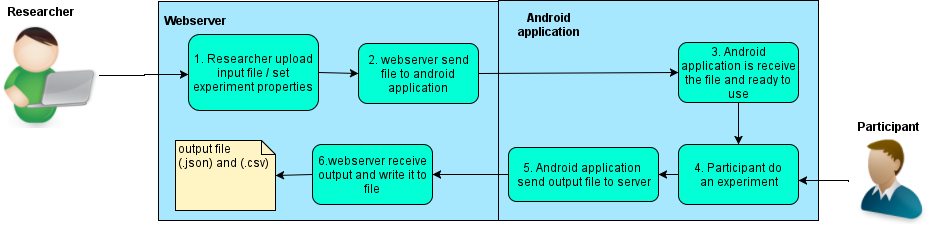
\includegraphics[width=\textwidth]{framework_process}
\centering
\captionsetup{justification=centering}
\caption{Flow of the experiment framework}
\label{fig:mainline}
\end{figure}

\subsection{Requirement}

Table \ref{tab:requirementList} below shows the list of all requirements of the application and its description.
% The main part are there are two
% main actors, a researcher and a participant. Researcher will able to set a input file and set parameters for the experiment. Participants then able to do the experiment by using the experiment application provided by the researcher. the application track the variables of the experiment. Finally, the researcher then able to download the experiment output\\

\begin{table}[!b]
  \centering
  \small
  \footnotesize
	\begin{tabu}{ |X[0.5,l]|X[5,l]|X[9,l]|  }
     \hline
     \multicolumn{3}{|c|}{Requirement List} \\
     \hline
     No& Name & Description \\
     \hline
     1   & Upload Input    & Researcher upload a JSON input file to the application\\ \hline
     2 & Download Output & Researcher download a JSON output file of the experiment\\ \hline
     3 & Insert multiple categories & Researcher insert multiple categories \\ \hline
     4 &  Insert questions & On each category researcher insert multiple questions\\ \hline
     5 & Set number of presented question & Researcher set how many question will be presented on each quiz phase   \\ \hline
     6 & Set presented question behavior &  Researcher set whether the number of presented question will be random each phase \\ \hline
     7 & Insert post question  &  Researcher insert the question that will be asked after the experiment, e.g demographic question \\ \hline
		 8 & Set experiment properties & Researcher able to set extra experiment's properties apart from input file.\\ \hline
		   9 & Insert notification  &  Researcher insert notifiaction and information on
       what is its content, when it will appear\\ \hline
       % and ow many millisecond  it takes to wait before shown to the user
      9 & See the questions  &  The participant can see the questions\\ \hline
      10 & Show answer link and answer page &  The participant can see and able to click the answer links  \\ \hline
      11 & Fill the answer  &  The participant can write an answer\\ \hline
      12 & Show notification  &  The application can show the notification \\ \hline
      13 & Track variables  &  The application can track defined variables\\
    \hline
    \end{tabu}
 \caption{List of requirements}
 \label{tab:requirementList}
\end{table}


\subsection{Input and Output}


The researcher needs to upload the input file that consists of all the experiment properties. After the experiment finishes, the result can be downloaded as a JSON file.
JSON (Java Script object notation) is used as an input and output format because it is very easy for a human to read and write, also for the machine to parse and generate.
Most of the current programming language and analysis software support JSON format \citep{jsonDesc}.
The JSON format consists of key and value pairs, on many programming languages it is similar to dictionary, table or struct. This input file will then be uploaded and compiled to the android application.
Here is a simple example of the JSON format.
To keep the data anonymous the researcher can set the participant id as empty, set parameter of experiment is explained on 4.2.3.
The application will generates a uique ID automaticaly that can be used
to identify the participant data.
%\hfill \break
%\newline
% \noindent\fbox{%
%     \parbox{\textwidth}{%
%        \{\\
%     \hspace{10mm}    name :"John",\\
%    \hspace{10mm}     age:21,\\
%     \hspace{10mm}    hooby:swimming\\
%        \}
%        }
%     }%
% \hfill \break
\begin{lstlisting}[language=json,firstnumber=1]
 {
    name:"John",
    age:21,
    hobby:"swimming"
 }
\end{lstlisting}
Table \ref{tab:inputFile} shows all the field for the input and its description. The output of the application will be a JSON file that consists of the experiment result
which consist of the answer to the all the questions and tracked variables.

\begin{table}[!tbh]
  \small
  \footnotesize
  \centering
\begin{tabu}{ |X[0.5,l]|X[6,l]|X[1.6,l]|X[7,l]|  }
 \hline
 \multicolumn{4}{|c|}{Input} \\
 \hline
 No& Name & Type & Description \\
 \hline
 1 & Study.PreText  & String & Html string that will be shown at first on the experiment\\  \hline
 2 & Study.PostText & String & Html string that will be shown after the pretext\\  \hline
 3 & Study.Name &  String & The name of the study \\  \hline
 4 & Study.Id & String & The Id of the study \\  \hline
 5 &  Experiment.Name & String & The name of the experiment \\  \hline
 6 & Experiment.NumQuestion & Integer & The amount of questions to be presented on each quiz phase \\  \hline
 7 & Experiment.MaxPresentedQuestion  & Integer &  The maximum number of presented question if it change randomly on each phase \\  \hline
 8 & Experiment.Random PresentedQuestion & Boolean &  Whether the number of presented question will be change randomly on each phase \\  \hline
9 & Category.Id  & String &  Id of the category \\  \hline
10 & Category.Name  & String & The name of the category \\
11 & Category.TotalQuestion & Integer  & The total size of the question on the category  \\  \hline
   12 & Category.QuestionOrder  &  String &  The order of how the question will be pulled from the list of questions.
   "LINEAR" it will be pulled based on the input order, "RANDOM" it will be pulled randomly\\  \hline
   13 & Category.Question.Id  &  String & The unique Id of the question \\ \hline
   14 & Category.Question.Text  & String &  The question text \\ \hline
   15 & Category.Question.linkAnswer  &  String & the URL link of answer \\ \hline
   16 & Category.Question.Answer  & String & the answer of the question \\ \hline
17 & Notification.App  & String & What application the phone will open if the participant click the notification \\  \hline
 18 & Notification.shift & Int &
 The number of phase when the notification should be shown. This will be explained more on the Notification section \\  \hline
 19 & Notification.Phase  & String & The activies name when the notification should be appeared\\  \hline
20 & Notification.TimeToShow & Integer  &  how millisecond the application should wait before showing the notification \\  \hline
 21 & Notification.Url  &  String & what url or id the application will open if the participant clicked the notification \\  \hline
 22 & Notification.TitleText  & String & The title of the notification \\  \hline
 23 & Notification.MsgText  &  String & The text of the notification  \\  \hline
\end{tabu}
\caption{Explanation of the entities inside the input file}
\label{tab:inputFile}
\end{table}

\subsection{Application Entities}
The input file that the researcher uploaded will be generated to an object.
The architecture of the object can be seen in figure \ref{fig:Experiment_objects}.
 Each box represents an object that consist of properties and methods.


 The biggest object is a \textit{study} object, this object is acted as a container for other objects.
The \textit{study} object holds another objects and control the flow of the experiment. The arrow in figure \ref{fig:Experiment_objects} represent which \textit{experiment}, \textit{category},
\textit{questions} and \textit{notification} will be used on the experiment. The \textit{study} object also acts as a tracker which will tracks variables during the experiment.

The \textit{experiment} object consists of properties on how the experiment will works, e.g experiment name, number of question will be asked, and how the question will be presented.
And each \textit{category} objects consist of \textit{questions} objects.

The researcher is able to choose which \textit{experiment} will be used and which \textit{notification} will be appeared.
While the participant can choose which \textit{category} they want to answered.
This selected \textit{experiment} and \textit{category} objects will be linked by
\textit{study} object and compiled as \textit{active category},\textit{active question} and \textit{active experiment}.

\begin{figure}[!b]
\begin{center}
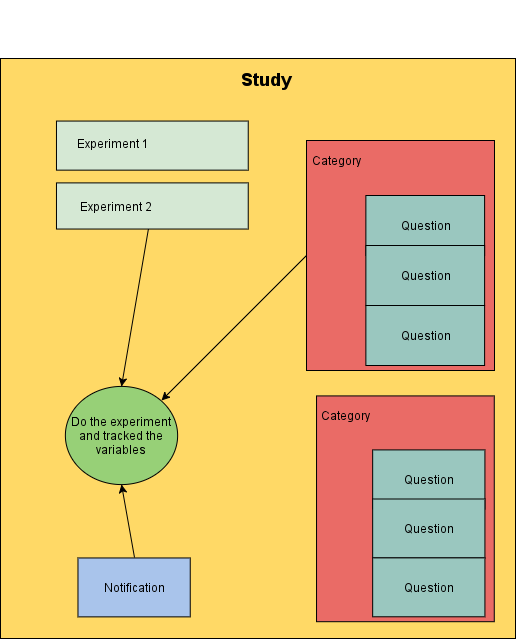
\includegraphics[scale=0.5]{quiz_Diagram}
\end{center}
\centering
\captionsetup{justification=centering}
\caption{Structure of the object inside the application}
\label{fig:Experiment_objects}
\end{figure}


\subsection{Application flow and properties}

The application has a general properties describe on table \ref{tab:variableList} which will be used to identify the status of the experiment.
These  also used to decide which notifications to show and what variables to track.

Figure \ref{fig:quiz_flowchart} shows the flow chart of the quiz experiment, and how the application  updated.
Figure \ref{fig:quiz_flow} shows the front end the application when the participant do the quiz experiment.

To make it easier for the reader the experiment's flow is divided into four stages;
\begin{figure*}[!b]
\begin{multicols}{2}
    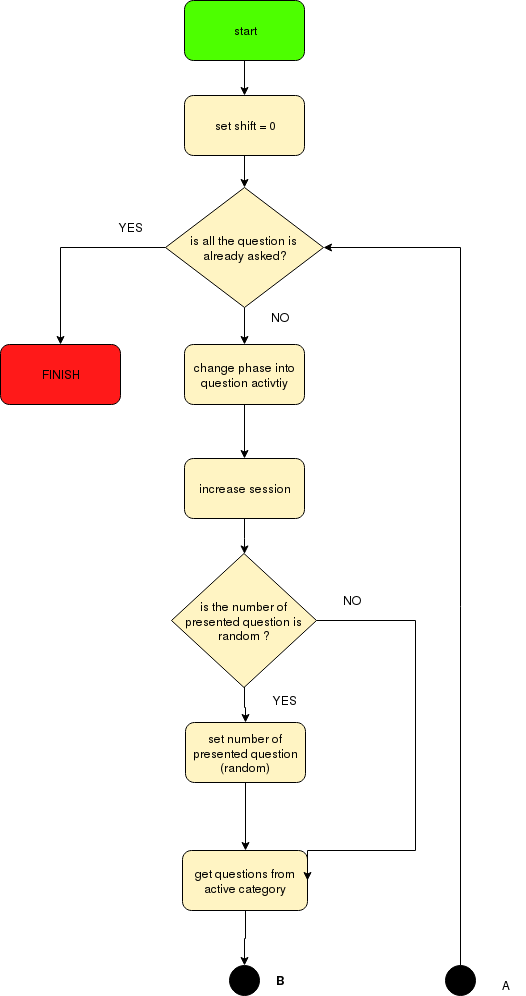
\includegraphics[scale=0.4]{Quiz_activity}\par
    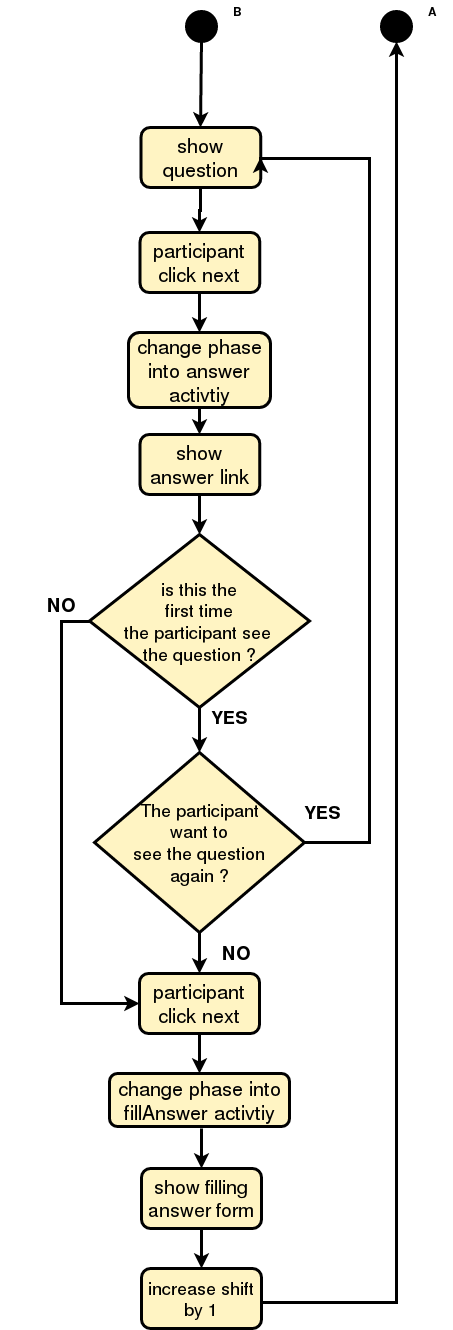
\includegraphics[scale=0.35]{Quiz_Activity_2}\par
    \end{multicols}
\centering
\captionsetup{justification=centering}
\caption{Quiz flowchart}
\label{fig:quiz_flowchart}
\end{figure*}


\begin{figure}[!t]
\begin{center}
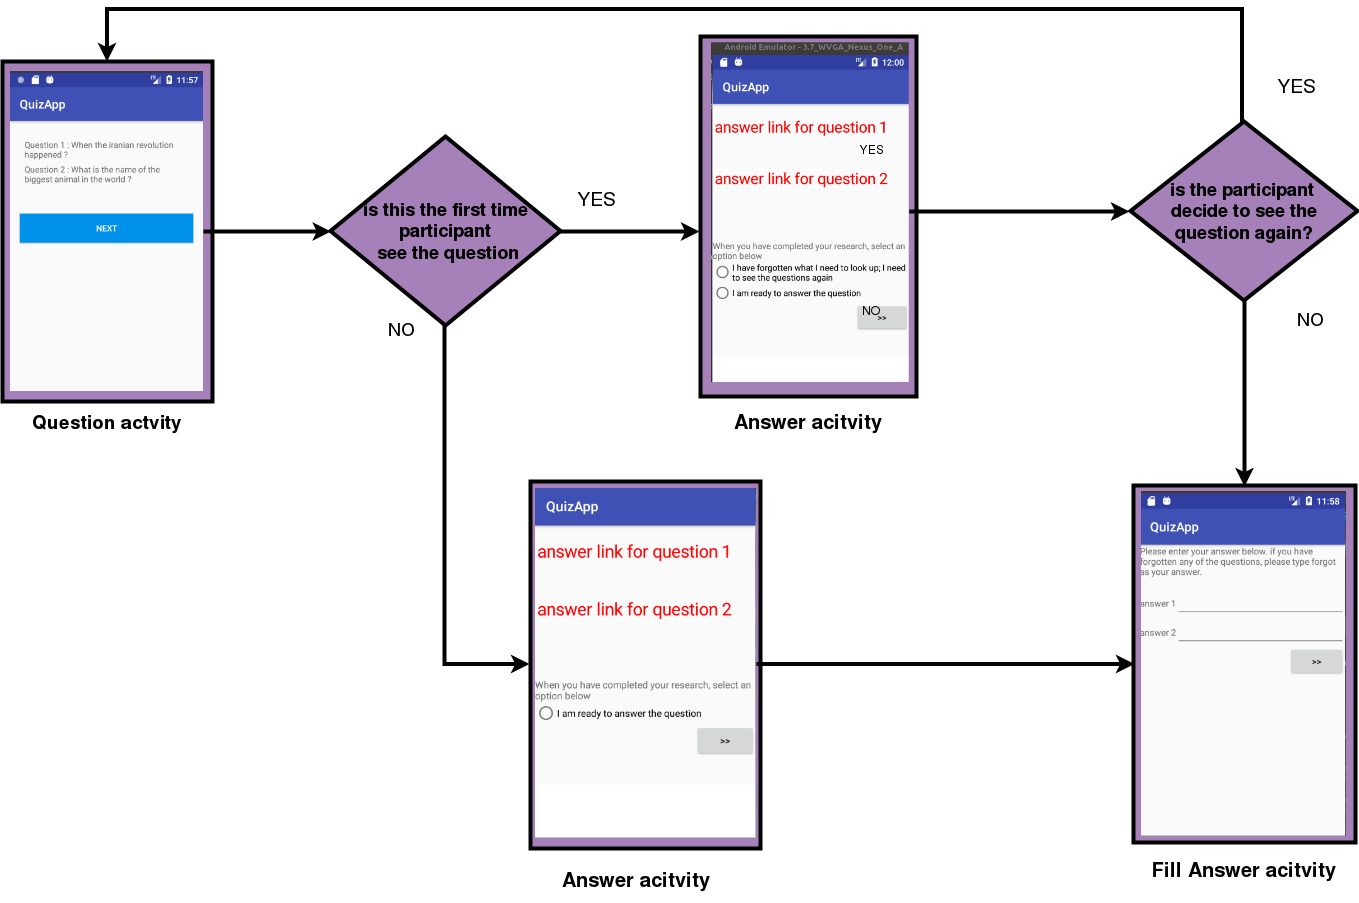
\includegraphics[scale=0.3]{Quiz_flow}
\end{center}
\centering
\captionsetup{justification=centering}
\caption{Front end of quiz activity flow}
\label{fig:quiz_flow}
\end{figure}

% \begin{itemize}
% \item \textit{Shift} : This variable is used to count how many question-answer had been done.
% \item \textit{Phase} : this variable has a value on what activity is currently active on the application
% \item \textit{Active Category} : The active category that will be choose by the participant during the experiment. This category will contain list of questions.
% \item \textit{Active Experiment} : This variable will contains the properties of the current experiment, this  set by the researcher from the application
% \item \textit{Number of presented question} : this variable value shows how many question are asked at one \textit{shift} of question-answer.
% \item \textit{Active Question }: the current question and it's answer link that is presented to the participant. This active question is picked from the question list inside the active category. the number of active question is based on \textit{number of presented question} variable.
% \end{itemize}

\begin{table}[!b]
  \centering
  \small
  \footnotesize
	\begin{tabu}{ |X[0.5,l]|X[3,l]|X[3,l]|X[7,l]|  }
		\hline
     No& Properties name & Type & Function \\
     \hline
     1   & \textit{Shift} & Integer & Used to count how many question-answer had been presented.\\ \hline
     2 & \textit{Phase} & String & What the name of activity that is currently active on the application.\\ \hline
     4 & \textit{Active Category} & Category & Contain category used in the experiment, and it contains list of questions.  \\ \hline
     5 &  \textit{Active Experiment} & Experiment & Contains the properties of the current experiment. \\ \hline
     %The  set by the researcher from the application.\\ \hline
     6 & \textit{Number of presented question} & Integer &  How many questions are presented at a time (\textit{shift}). \\ \hline
7 & \textit{Active Question } & List of Question & List of the question that is presented to the participant. \\
                        %This variable is picked from the question list inside the active category.\\
\hline
    \end{tabu}
    % \centering
    % \captionsetup{justification=centering}
 \caption{List of general properties of the experiment}
 \label{tab:variableList}
\end{table}



\begin{itemize}
\item \textbf{Initialization} : firstly a \textit{phase} variable is initialize. The application then confirm if the experiment is active by ensuring that there is still questions need to be asked. The quiz is finished if all the question has been asked.
\item \textbf{Question activity} :  The number of presented question is changed (randomly or constant).
Then questions are picked from the \textit{active category} and put to \textit{active question}. Then the \textit{active questions} are presented to the participant.
\item \textbf{Answer activity} : Thirdly, the links for the answer page are presented to the participant. The participant then click the links and find the answer inside the answer page.
The participant is able to see the question again or decide to answer. The participant is only allowed to see the question again one time.
\item \textbf{fill answer activity} Lastly, the participant need to write the answer to the question on the text box.
After that, the \textit{phase} variable is increased and the application will repeat the quiz again until it finished.
\end{itemize}


\subsection{Notification Design}

During the quiz experiment the notification will be shown to the participant.
Notification will be shown as a pop-up box as seen in figure \ref{fig:clicked_notification_flow}.
When the notification is shown to the screen, the phone will vibrate and produce a sound.

 If the participant click the notification then the application will be minimized and the android phone will be directed to another application.
 After that, the user can click the application icon to get back to the experiment application.

Based on this design, the \textit{notification} should have the properties listed on table \ref{NotifactionProperties}.
% \begin{itemize}
% \item \textit{shift} : This property is to decide on which shitft the notification will be shown, it will be compared to the \textit{shift} properties of the study object.
% \item \textit{phase} : This  to decide on which activity (question, answer and fill answer) the notification will be shown.
% \item \textit{app} : What application the notification will open, it also need to have a value of the user or url of the application.
% \item \textit{timeToshow} : How millisecond the framework should wait before the notification will be shown
% \item \textit{notification text} : What is the message text inside the notification box
% \end{itemize}

\begin{table}[!b]
\centering
\small
\footnotesize
\begin{tabu}{|X[2,l]|X[5,l]|}
\hline
Variable          & Function                                                                                                                                  \\ \hline
shift             & This property is to decide on which shitft the notification will be shown, it will be compared to shift variable in experiment properties \\ \hline
phase             & This  to decide on which activity (question, answer and fillanswer) the notification will be shown.                          \\ \hline
app               & An application the notification will open; instagram, twitter, facebook or website.                           \\ \hline
timeToshow        & Time (in millisecond) notificationwill the notifiaction need to wait before presented.                                                           \\ \hline
notification text & The message text inside the pop-up box                                                                                     \\ \hline
\end{tabu}
% \centering
% \captionsetup{justification=centering}
\caption{The properties of notification object}
\label{NotifactionProperties}

\end{table}


\begin{figure}[!b]
\begin{center}
\fbox{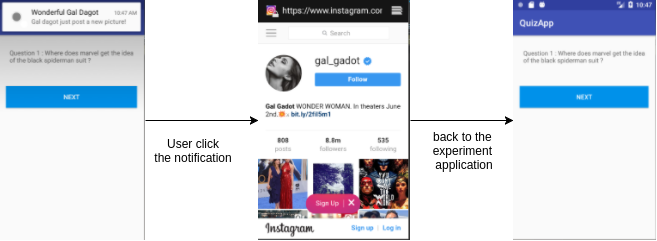
\includegraphics[scale=0.65]{notication}}
\end{center}
\centering
\captionsetup{justification=centering}
\caption{Flow of the notification}
\label{fig:clicked_notification_flow}
\end{figure}



\subsection{Tracked Variable}
During the experiment the application track variables. Table \ref{tab:trackedVarible} consist of all the variables that the application track.
some of the variables have \textbf{lb} in front of their name, this mean that variable is tracked during the lookback process.
A process when the participant look the question again for the second time.

\begin{table}[!b]
  \centering
  \small
  \footnotesize
\begin{tabu}{ |X[0.3,l]|X[2.3,l]|X[0.9,l]|X[5,l]|  }
 \hline
 \multicolumn{4}{|c|}{Tracked variables list} \\
 \hline
 No & Variable's name & Type & Description \\
 \hline
 1 & TTLQ & Long  & total time (in millisecond) when the participant see the question until they click next button\\ \hline
 2 & lb\_TTLQ & Long & similar with TTLQ, but after lookback\\ \hline
 3 & LookBack & Boolean & \textbf{True} if the participant decide to look at the question again, \textbf{false} otherwise. \\ \hline
 4 & TTLB & Long & total time (in millisecond) when the participant see the answer links until they click the next button (to look the question again or answer the question) \\ \hline
 5 & lb\_TTLB & Long & Similar with TTLB, but after lookback\\ \hline
 6 & visited\_links & List of String & The list of links clicked/visited by the participant after clicking the answer links\\ \hline
 7 & time\_visited\_links & List of Long  & List of the total time (in millisecond) the participant spent on each asnwer page\\ \hline
 8 & lb\_visited\_links & List of String & Similar to visited\_links, but after lookback\\ \hline
 9 & lb\_time\_visited\_links & List of Long & Similar with time\_visited\_links, but after lookback\\ \hline
 10 & TTLA & Long & Total time (in millisecond) the participant spent writing the answer\\
 11 & TTLFA & Long & Total time (in milisecond) the participant write the answer on the text box\\ \hline
 12 &  num\_notif & Integer & how many notification is shown during the a question \\ \hline
 13 & TTLN & Long & Total time (in millisecond) it tooks the participant after clicking the notification to back to experiment application\\ \hline
 \end{tabu}

%
%  \hline
%  \end{longtable}
\caption{List of tracked variable}
 \label{tab:trackedVarible}
\end{table}
\par




\chapter{Implementation}
This chapter discussed the technical implementation of the system based on the design discussed before.
Section 4.1 provides the technical information about the main entity as classes that will be used in this study, including its variables and methods.
Section 4.2  provides a complete information about the work flow of the application.
Section 4.3 provides an information about the mechanism of notification. Lastly, section 4.4 provides an information about the tracker and its procedure.

Flask framework and python programming language is used to develop the webserver. Java programming language and Android SDK is used to develop android application.

% \subsection{Web server}
% explain sending data to the android application
% Webserver is a http server that
% send a json file


%explain get data from android appplication


\section{Entities relationship}
All the entities discussed in the design chapter will be represented as a class which consists of variables and methods.
The relationship between classes can be seen on the class diagram on figure \ref{fig:class_diagram}.
 The box presents the class. The upper part of the box consists of the variable name and its type.
 The plus and minus sign before the variable name present the scope of the variable.
  Minus (-) means private and plus (+) means public.
  The bottom part of the box consists of the class methods and the type of its output.
  Furthermore, the arrow presents the variable relationship whether it can be one-to-one (1..1)  or one-to-many(1..*) relationship.
  The arrow also present that a class extend other class which means it has same properties and methods.

\begin{sidewaysfigure}[ht]
\begin{center}
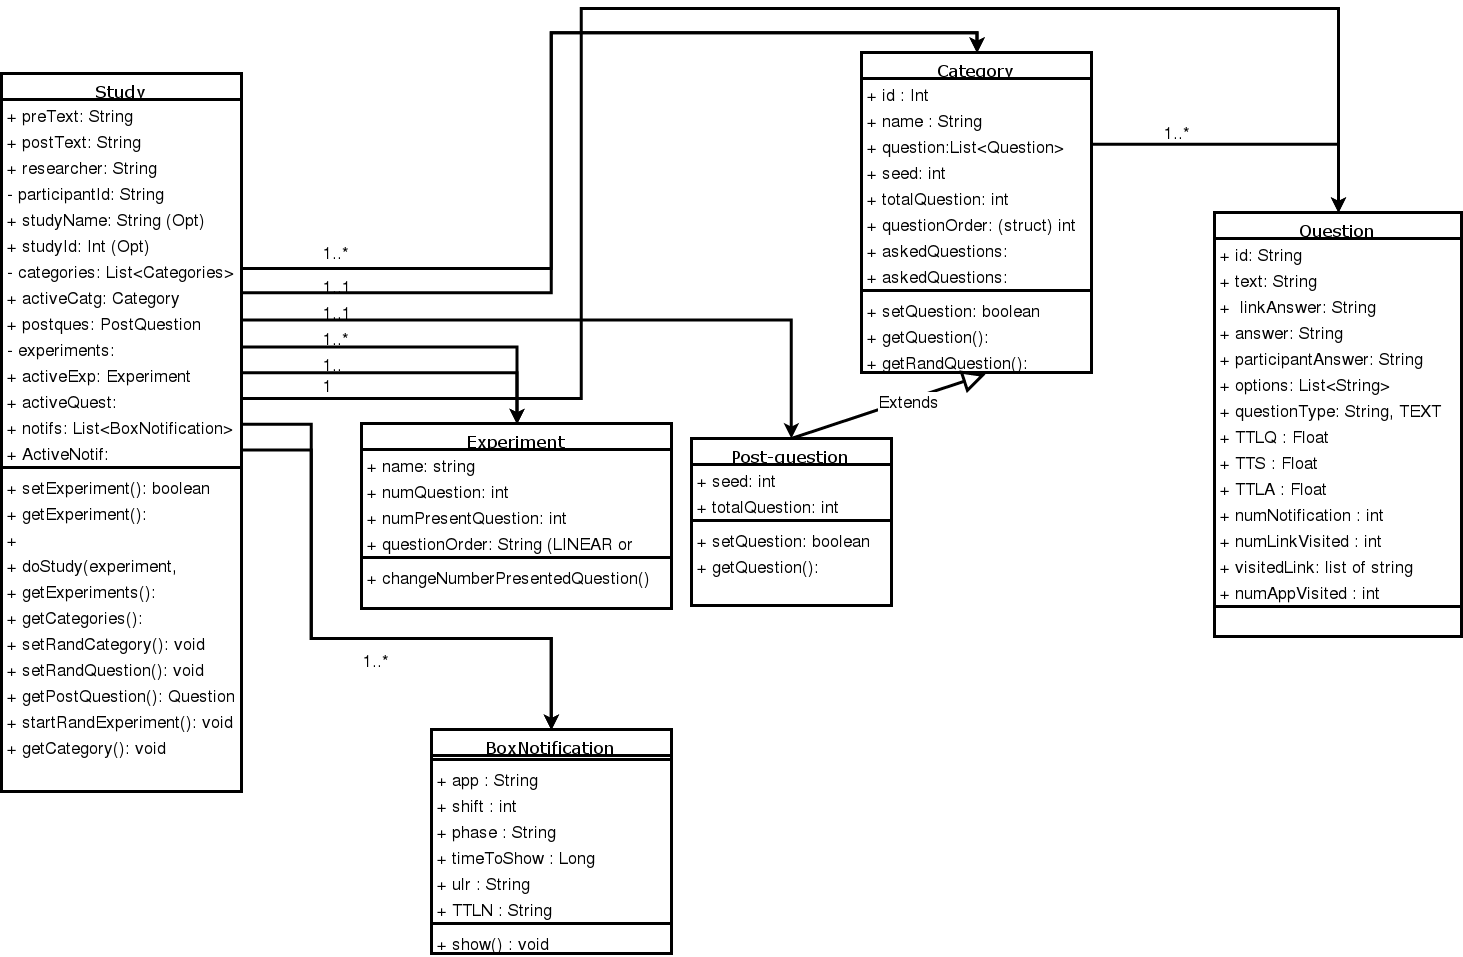
\includegraphics[scale=0.3]{class_diagram}
\end{center}
\caption{Class diagram of the application}
\label{fig:class_diagram}
\end{sidewaysfigure}

\subsection{Study Class}
Study class is the class that acts as a central container for other entities of the application, and it controls the flow of the main function of the experiment.
Some of its properties are defined from an input file; \textit{preText, postText, researcher, studyName, studyId}.
As seen in the class diagram \ref{fig:class_diagram}. The study class contains \textit{experiments} variable which consists of a list of experiment objects.
 \textit{Categories} variable which consists of a list of category objects, and \textit{notifs} variable that consists of a list of notification objects.

As explained in the design section, the experiment application need to initialize following variables before conducting the experiment;
\textit{ActiveExp} (active experiment) variable is experiment that will be conducted, and \textit{activeCatg} (active category) is the
category that will be used to pick questions.
\textit{ActiveQuest} (active question) variable present what questions are currently asked to the participant.
The question inside \textit{activeQuest} variable are picked from the a list of questions inside the active category (\textit{activeCatg}) variable.
\textit{ActiveExp} is set by the researcher on the setting experiment window, and the \textit{activeCatg} is chosen by the participant during the experiment



%After the category (\textit{activeCatg}) and set the experiment %(\textit{activeExp}) are chosen, the experiment can be started. The experiment will present the participant with one or several questions. In the study class there is \textit{activeQuest} (active question) variable that contains the  question objects that is being on a \textit{shift}.

Moreover, the class also contains \textit{activeNotif} (active notification) variable.
This variable contains a list of notifications that have been presented to the participant.
The notification object is picked from the \textit{notifications} variable that contains all the notification.

% \begin{table}[!b]
%   \centering
%   \begin{longtable}{ |p{0.5cm}|p{4cm}|p{2.3cm}|p{6cm}|  }
%  \hline
%  No& Variable's name & Type & Description \\
%  \hline
%  1 & preText & string  & the text\\
%  2 & postText & string & THIS DESCRIPTION NEED TO BE FILLED\\
%  3 & researcher & string & True if the participant decide to look at the question again, false otherwise. \\
%  4 & studyName & string & total time (in millisecond) when the participant see the answer links and decide to look the question again or answer the question (next button) \\
%  5 & studyId & string & Similar with TTLB and the participant decide to look at the question again.Then, answer links are shown again to the participant\\
%  6 & participantId & List of String & The list of links clicked/visited by the participant after clicking the answer links\\
%  7 & randomGenerator & List of Long  & List of the total time (in millisecond) the participant stay on a page after clicking link\\
%  8 & categories & List of String & similar with visited\_links but the participant have decided to see the question again then return to the answer links window\\
%  9 & experiments & List of Long & Similar with time\_visited\_links but the participant decide to look at the question again then click the answer links\\
%  10 & postques & Long & Total time (in millisecond) the participant see the fill answer window and then click next\\
%  11 & activeExp & Long & Total time (in milisecond) the participant write the answer on the text box\\
%  12 &  activeCatg & Integer & how many notification is shown during the a question \\
%  14 & activeQuest & Long & Total time (in millisecond) it tooks the participant after clicking the notification to back to experiment application\\
%  15 & notifs & Long & Total time (in millisecond) it tooks the participant after clicking the notification to back to experiment application\\
%  16 & activeNotif & Long & Total time (in millisecond) it tooks the participant after clicking the notification to back to experiment application\\
%  16 & shiftNum & Long & Total time (in millisecond) it tooks the participant after clicking the notification to back to experiment application\\

% \hline
% \end{longtable}
% \caption{Variable inside study class}
%  \label{tab:studyClassVariable}
% \end{table} \par
\subsection{Experiment Class}
The Experiment class contains the \textit{experiment variables} that is used to define the behaviour of the experiment.
The variables are explained in the table \ref{tab:ExperimentClassVariable}.
Every variables inside this class except \textit{numPresentedQuestion} is determined from the input file. \textit{numPresentedQuestion} is a variable that
control how many questions is presented to the participant each time.
 \textbf{changeNumberPresentedQuestion()} method is called by the study class to change the value \textit{numPresentedQuestion} variable.
 The change can be random (from 1 to \textit{maxPresentedQuestion}) by using the Random object (RandomGenerator)
  provided by Java API.

\begin{table}[!htb]
  \centering
  \small
  \footnotesize
\begin{tabu}{|X[0.5,l]|X[5,l]   |X[2.3,l]|X[6,l]|  }
 \hline
 No & Variable's name & Type & Description \\
 \hline
 1 & name & string  & The name of the experiment\\ \hline
 2 & numQuestion & Integer & The number of questions will be asked on the experiment \\ \hline
 3 & numPresentedQuestion & Integer & The number of question presented to the participant on the experiment every phase of question-answer \\ \hline
 4 & questionOrder & String & If the value is RANDOM, then the question is picked randomly from a list of question, if the value is LINEAR then the question will be picked based on the order of the input file \\ \hline
 5 & randomPresentedQuestion & Boolean & If it the value is true, then on each phase the num of presented question will change randomly, explained more on changeNumberPresentedQuestion method \\ \hline
 6 & maxPresentedQuestion & Integer & This is the maximum number of presented question if the number of presented question is decided randomly\\ \hline
 7 & randomGenerator & Random  & This is a random class that use to generate random number, it is used inside changeNumberPresentedQuestion method \\ \hline
\end{tabu} \par
\caption{variables inside the experiment class}
 \label{tab:ExperimentClassVariable}
\end{table}

\subsection{Category Class}
Category class is used to carry the questions objects.
It has two main variables; \textit{questions} and \textit{askedQuestion}.
\textit{Questions} variable consist a list of questions. This variable is filled by
the question from the input file.
\textit{AskedQuestion} variable consists of all the question that had been asked.

The class has two main methods \textit{getRandQuestion()} and \textit{getQuestion()}.
These methods will be called during the quiz activity to put question object into activeQuestion variable.
These methods are two different procedure to pick a question from \textit{questions} variable.
the former takes the question randomly while the latter takes the question based on the order of the input file.
Java random class is used to generate random index (from 0 to the size of the \textit{questions} variable).
After the question is selected, it will get deleted from the \textit{questions} variable and then it will be put it into \textit{askedQuestion} variable.

\subsection{Question Class}
Table \ref{tab:questionClassVariable} shows the variables inside this class.
The \textit{question} class consist of the content of question; its question text, answer link and answer.
The class also contains the tracked variable (the variables are explained more on trackker section).
The question can be two type MC or TEXT. MC means multiple choice, this question type will have multiple options on its answer choice,
and the participant can chose one of them. while TEXT means that the participant need to write the question.
\textit{representId} is generated when the questions are presented to the participant. this variable is unique and can
be used to classify which questions are presented at the same time.

\begin{table}[!tbh]
  \centering
  \small
  \footnotesize
  \begin{tabu}{|X[0.5,l]|X[4,l]|X[2.3,l]|X[6,l] |}
 \hline
 No & Variable's name & Type & Description \\
 \hline
 1 & id & string  & The id of the question.\\  \hline
 2 & text & string & The text of the question.\\ \hline
 3 & linkAnswer & string & the URL link to the answer page. \\ \hline
 4 & answer & string & (optional) the answer of the question. \\ \hline
 5 & participantAnswer & string & the answer of the participant during the quiz activity.\\ \hline
 6 & questionType & String & The type of the question. The value can be "MC" or "TEXT".\\ \hline
 7 & representId & string  &  the random id generated when the question is presented during quiz.\\ \hline
 7 & options & list of String  & The answer option if the question is multiple choice.\\ \hline
\end{tabu}
\caption{Variable inside Question class (without the tracked variable)}
 \label{tab:questionClassVariable}
\end{table} \par

\subsection{BoxNotification class}
BoxNotification is used as a class name because the name Notification is already defined inside the Android framework.
Most of the variable in this class is similar to the defined variable in the design section.
Similar to the question class, the notification also contains \textit{presentedID} which show
on which question the notification is shown.
The content of the notification can be set into \textit{title} and \textit{msgText} variable.
The Notification can open an android application of twitter, facebook, instagram and web browser. The application should be installed on the phone, otherwise, the notification will open the url of the application on the web browser.
To define which user will be shown if the user clicked the instagram, twitter or facebook notification. The user
is defined by the user\_id code which can be found on the profile of their social media.
the url can also contain the URL link, then the application will open the web page.
This app needs to be specified on the \textit{app} variable and the \textit{url} variable. The \textit{url} variable needs to be filled with the user id of the twitter or instagram. Or it can be filled with http/https url to open web page. the class contains a show() method that will pop up the notification in the android phone.
The mechanism and flow of the notification will be explained on next chapter.

%
% \begin{table}
%   \centering
%   \small
%   \footnotesize
% \begin{tabu}{ |X[0.5,l]|X[4,l]|X[2.3,l]|X[6,l]|  }
%  \hline
%  No& Variable's name & Type & Description \\
%  \hline
%  1 & url & String & this contains  \ \hline
%  2 & titleText & Integer & this is the maximum number of presented question if the number of presented question is decided randomly\\ \hline
%  3 & msgText & Random  & this is a random class that use to generate random nunmber, it is used inside changeNumberPresentedQuestion method \\ \hline
%  4 & presentedID & Random  & this is a random class that use to generate random nunmber, it is used inside changeNumberPresentedQuestion method\\
% \hline
% \end{tabu}
% \caption{variable inside notification class, some of the variable are already discussed on the design section}
%  \label{tab:NotificationVariable}
% \end{table}

\section{Application flow}
In this section, the flow of the application from the technical point of view is provided.
The flow of the application can be seen
on figure \ref{fig:flowOfApplication}. The figure shows the flow of the application after input file is uploaded and
the experiment just has started.
As it seen in figure, the flow is divided into four scopes;
\begin{itemize}
\item \textbf{Setting}  : the researcher can set some properties of the experiment or choose to start the experiment.
\item \textbf{Experiment} : The participant conducts the quiz experiment.
\item \textbf{Notification} : The notification can be shown during the quiz.
\item \textbf{PostQuestion} : The participant presented with post questions.
\end{itemize}
\par

To have a further understanding about the application flow, the activities and method on the flow chart are explained further in the following subsection.



\begin{figure}
\begin{center}
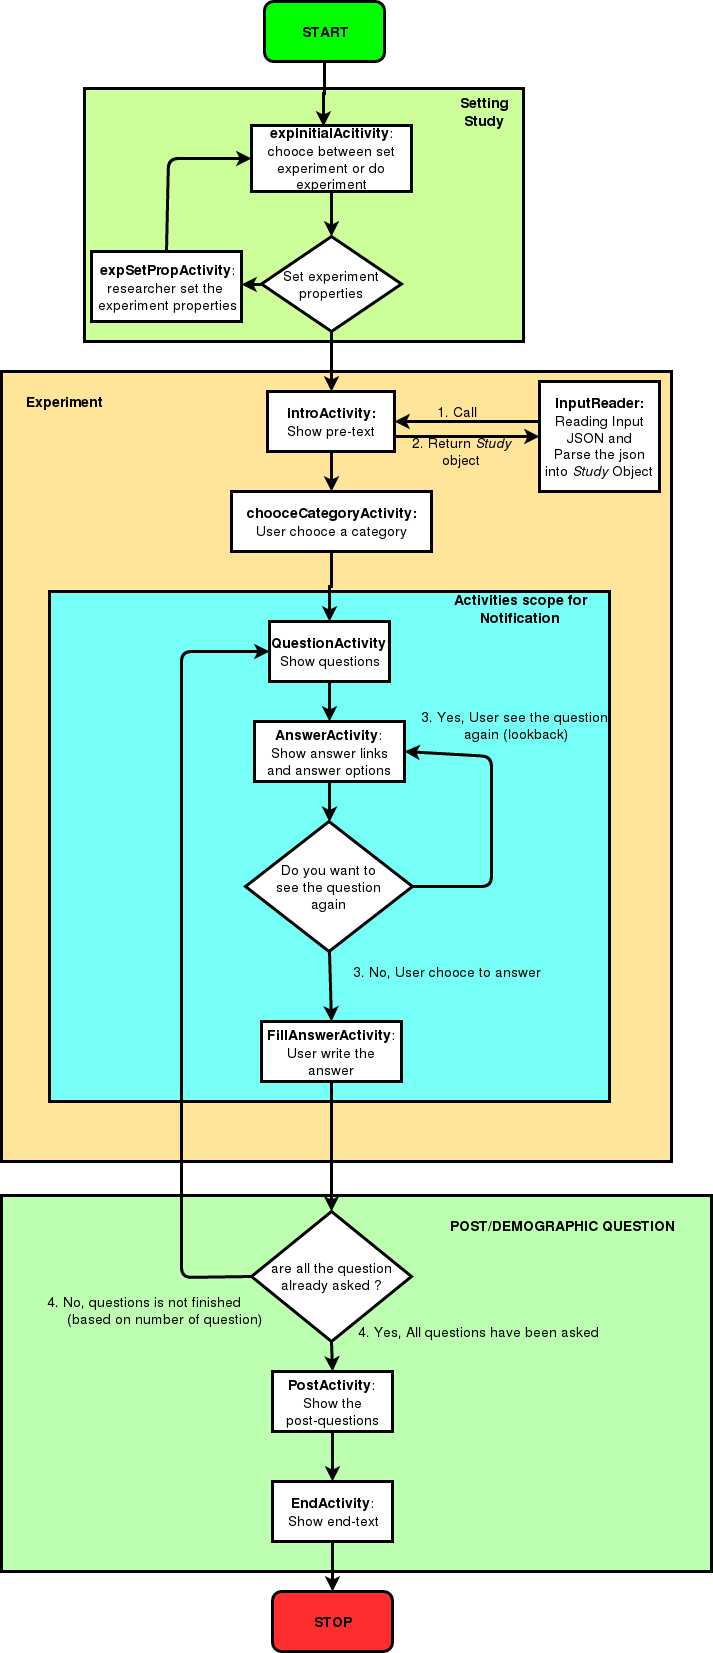
\includegraphics[scale=0.4]{Flowchart_}
\end{center}
\centering
\captionsetup{justification=centering}
\caption{The flow of the application}
\label{fig:flowOfApplication}
\end{figure}

\subsection{Android Activity}
The android application built upon multiple class activities.
Each activity has a user Interface (UI) template. this template is saved into an xml file. The template consists of UI element, for example, button, text, etc.
Its corresponding class activity will decide what will appear on the phone or what happens if a button is clicked.
For example, answerActivity class will have activity\_answer.xml template.
The activity class is used to catch the event such us clicked or move to another application. This event is linked to an \textit{event listener} methods.

The android application also contains a lifecycle which is default methods and activities that will be called every time.
Figure \ref{fig:theLifeCycleOfActivity} shows the android activity lifecycle \citep{androidActivity}.
There are three methods inside the lifecycle that is used in this experiment application;
 \textit{OnCreate()} is the first method to get called every time the activity start.
 \textit{OnPause()} will be called if the phone move to another application.
 Lastly,  \textit{OnResume()} is called if the user open the application again after leaving the application.

\begin{figure}[!tbh]
\begin{center}
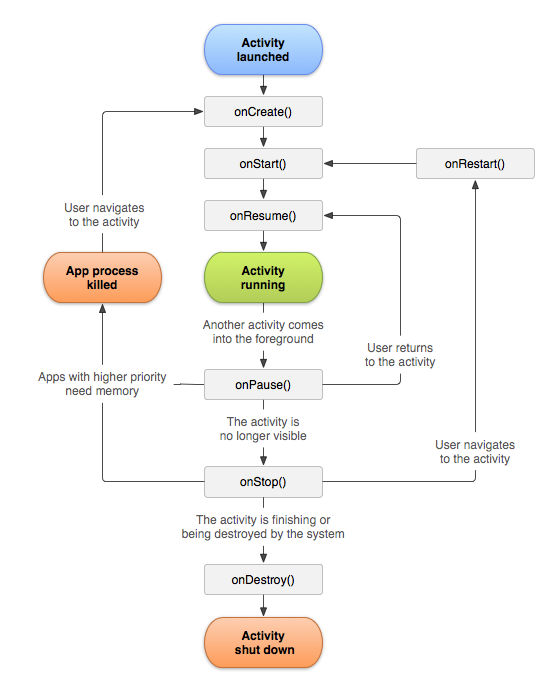
\includegraphics[scale=0.5]{activityLifeCycle}
\end{center}
\centering
\captionsetup{justification=centering}
\caption{The lifecycle of android application}
\label{fig:theLifeCycleOfActivity}
\end{figure}



\subsection{expInitialActivity}
The UI layout of this activity can be seen in figure \ref{fig:expInitialActivity}.
The participant can click a button to begin the experiment or to set the properties of the experiment.
On the \textbf{OnCreate()} method the \textbf{InputReader.read()} method is called firstly.
This method will read the JSON input and compiled it into \textit{Study} object.
String input is compiled into JSON object by using \textit{GSON} library.
\textit{GSON} is a serialization / deserialization library that is used to convert a string into a JSON object or another way around. \citep{gsonLib}

Then the JSON object compiled into The \textit{Study} object. This object controlled the quiz experiment and hold all the data, including the track variables.
This object will be sent through the activities.
\textit{Intent} class of java is used to encapsulate the object and send to another activity.
Because the \textit{Study} object need to be encapsulated inside the Intent,
 java programming language requires every class including the Study class to implement \textit{Serializable}.

%
% \begin{figure*}
% \centering
% \begin{minipage}[b]{.4\textwidth}
% 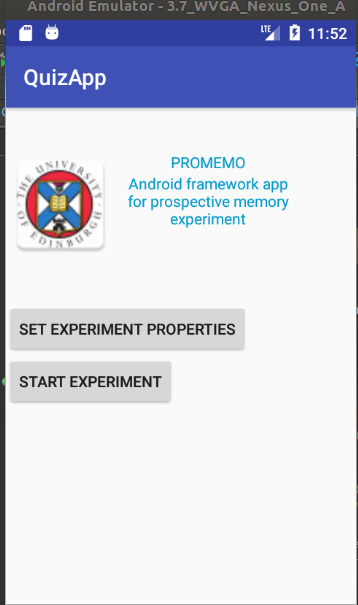
\includegraphics[scale=0.32]{FE_1}
% \caption{Caption}\label{label-a}
% \end{minipage}\qquad
% \begin{minipage}[b]{.4\textwidth}
% 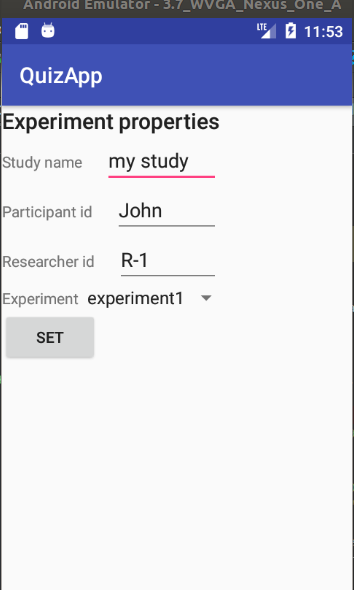
\includegraphics[scale=0.32]{FE_set_properties}
% \caption{Caption}\label{label-b}
% \end{minipage}
% \end{figure*}

\subsection{expSetPropActivity}
The UI layout of this activity can be seen in figure \ref{fig:expSetPropActivity}.
This activity is used to set some parameter of the experiment. In this activity the researcher can pick which experiment to conduct, the name of the experiment,
the id of the researcher and the id of the participant.
The purpose of this activity is to make it easier for the researcher to conduct multiple experiments and multiple participants without uploading the input file again.

\subsection{IntroActivity}
The UI layout of this activity can be seen in figure \ref{fig:IntroActivity}.
This activity is used to show the information about the experiment to the participant before starting the experiment.
This information is obtained from the preText and postText variables. the value of this variable will be converted into a html and shown to the participant.
Figure X show example of the Consent information shown inside the application.

\subsection{ChooseCategoryActivity}
The UI layout of this activity can be seen in figure \ref{fig:ChooseCategoryActivity}.
In this activity the participant chooses which category he/she want to answer.
The selected category name will then save in the \textit{selectedCategoryName} variable inside study class.
\textit{selectedCategoryName} is used to in the experiment initialization to initialize \textit{activeCatg} variable


\subsection{QuestionActivity}
The UI layout of this activity can be seen in figure \ref{fig:QuestionActivity}.
In this activity, the question inside \textit{activeQuestion} variables is shown to the participant.
This activity will be called multiple time during the quiz experiment.
the main function of this activity is to call \textbf{Study.runExperiment()} method.
\textbf{Study.runExperiment()} is used to start or continue the quiz experiment.
this method is explained in the section below.

\subsubsection{Study.RunExperiment()}
This method will be called everytime the Quiz activity started.
The main function of this methods are :
\begin{itemize}
\item Initialize the active experiment (\textit{activeExp} variable) and active category (\textit{activeCatg}) variable.
\item Change the number of \textit{presentedQuestion} (the variable is explained in the Experiment class section).
\item Set the active questions (\textit{activeQuest}) from the questions in the category.
\end{itemize}


\begin{figure}
\begin{center}
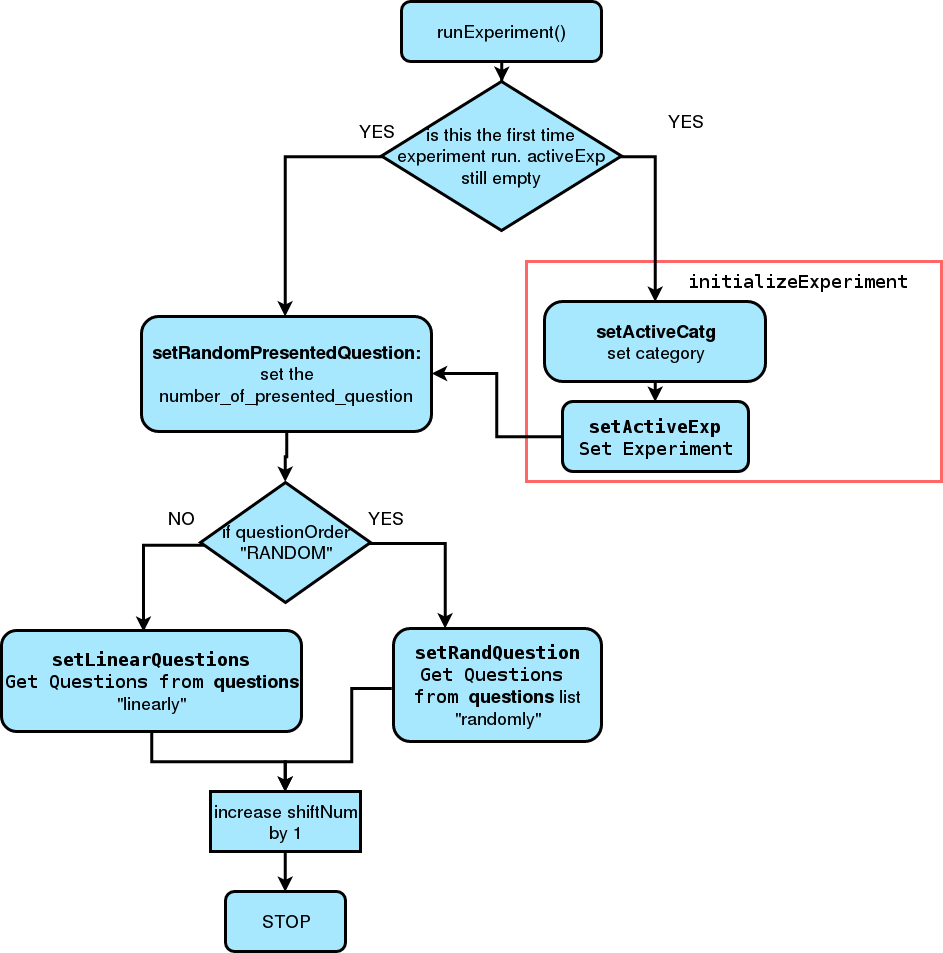
\includegraphics[scale=0.45]{runExperiment}
\end{center}
\caption{Flow chart of runExperiment method}
\label{fig:runExperiment_flow}
\end{figure}


Figure \ref{fig:runExperiment_flow} shows the work flow of the method. The First step is to initialize the experiment by checking the active experiment (\textit{activeExp}) variable.
   if it's empty then it's the beginning of the experiment, hence some variables needs be initialized. If it's mean that the experiment had been started (on-going)
 so new question is presented to the participant.


On the inisialization, active experiment (\textit{activeExp}) and active category (\textit{activeCatg}) are initialized by calling \textbf{initializeExperiment} method.
The \textbf{initializeExperiment} method will fetch the selected \textit{experiment} and the
\textit{category} object from the study class variables based on the \textit{selectedExperimentName} and \textit{selectedCategoryName}.


Subsequently, the \textbf{setRandomPresentedQuestion()} is called, this method will set the value of \textit{numPresentedQuestion}.
If the researcher set randomPresentedQuestion to true in the input file, then \textbf{Experiment.changeNumberPresentedQuestion()} is called, this method will set numPresentedQuestion randomly
On the other hand, if it's false, then the numPresentedQuestion will be constant.

Next, \textbf{isExperimentIsStillGoing()} is called. This method make sure if the experiment is still on progress by checking the size of the
\textit{question} variable inside the \textit{activeCatg}. If the size is still larger or similar then \textit{numPresentedQuestion} then the experiment can be continued.

Lastly, the active question (\textit{activeQuest}) is picked from the questions variable by calling \textbf{setActiveQuestion()}. this method filled
 i \textit{activeQuest} variable by fetching \textit{question} object from the \textit{question} variable inside \textit{activeCatg} object.
  The question object will be picked randomly if the researcher set \textit{questionOrder} to random. Otherwise, it will be picked linearly based on
  the input file order.


\subsubsection{AnswerActivity}
The UI layout of this activity can be seen in figure \ref{fig:AnswerActivity}.
In this activity, the answer links are shown as a textview inside the UI layout. If the participant clicks the answer
link then the \textbf{clickListener()} method inside the textview will open the answer page.
A java class called \textit{webview} is used as a browser. The \textit{webview} will open the web page based on the URL of the answer link (\textit{question.url}).

On the layout, two radio buttons are presented to the participant. These are the option whether the participant wants to return to see the question again or to continue
 to answer the question.
If the participant chose to look at the question again then a special string is capsulated inside the \textit{intent} object.
This string is sent to question activity then send back to answer activity. this string is used to indicate if the participant looks at the question again.
If the string is sent to answerActivity then the radio button "to see the question again" is hidden.


\subsection{fillAnswerActivity}
The UI layout of this activity can be seen in figure \ref{fig:fillAnswerActivity}.
In this activity, the participant should answer the question by writing the answer on the editText UI.
If the participant clicks next button then \textbf{saveAnswer()} method is called. this method will get the value of the editText
and stored it on the \textit{participantAnswer} variable inside the \textit{question} object.


\section{Notification mechanism}
Figure \ref{fig:NotificationFlo} shows the mechanism of notification.
As seen on the flowchart, the \textbf{checkNotification()} method is called inside
the OnCreate event on the QuestionActivity, AnswerActivity and FillAnswerActivity.
The method checks on every notifications inside the \textit{notifs} variable if the there is a notification that should be shown up based on \textit{phase} and \textit{shift} variable of the notification.

If there is a notification that needs to be shown up then the notification object is added into the \textit{activeNotif} and it is deleted from the \textit{notifs} variable of the study object.

The notification needs to wait for some millisecond before it can be shown up. The waiting time is defined in \textit{timeToshow} variable inside the BoxNotification class.
While the notification process waits, the main activity should keep working, so another process needs to be spawned a part of the main process.
To accomplish it, \textit{TimerService} class is used. This class will be spawn as a new process and it will sleep for \textit{timeToShow} millisecond.
After that, the service class will call the \textbf{BroadcastReceiver()}.
The \textbf{BroadcastReceiver()} method  is defined on all of activities, and it simply calls \textbf{show()} method of the notification.
The \textbf{Notifaction.show()} method is used to show the notification to the front end of the android screen. This method use
 \textit{NotificationCompact.Builder} to build the notification layout.
 an \textit{Intent} object is inserted inside the Builder object that contains what application to open.
 If the participant clicks the notification then the experiment application will be minimized.
 This event will call \textbf{OnPause()} method on the current activity, and the android phone will open the intended application.
 The participant if the open the experiment application again, then the \textbf{OnResume()} method is called.


\section{Tracker}

The tracked variable are shown on the table \ref{tab:trackedVarible}.
All of these variable are stored inside the \textit{question} class as seen in the class diagram \ref{fig:class_diagram}.
Some of the variables are used to track the time in millisecond.
To track the time the \textit{stopWatch} class provided by java API is used.
The StopWatch object is stored inside the study class because the StopWatch class is not serizable.
During the experiment the application is minimized (participant clicks the notification).
Then event some Stopwatch object need to be paused. Inside \textbf{OnPause()} event listener the stopWatch is suspended,
and it will resume again inside the \textbf{OnResume()} event listener.

As seen in the class diagram, each one of tracked variable has its own \textit{stopWatch} object, for example \textit{stopWatchTTLQ} will track the time for TTLQ variable.
To get the millisecond time of the stopwatch a \textbf{StopWatch.getTime()} method is called.
Then to stored the tracked time, the \textbf{study.log()} method is called.
This method pass two arguments; what variable to track and which stopwatch object is used to track it.
for instance \textbf{study.log("TTLQ",stopWatchTTLQ)} will track the \textit{TTLQ} variable and use \textit{stopWatchTTLQ} to track the time.
All of the tracked variable is then stored to the \textit{question} object inside the \textit{ActiveQuest} variable.
How each variable is tracked is explained further in the subsection below.
The explanation of the variables are explained on table \ref{tab:trackedVarible}.

\subsubsection{TTLQ, lb\_TTLQ and lookback}
These variables is tracked inside the \textit{questionActivity}.
\textit{StopWatchTTLQ} and \textit{stopWatchTTLQ\_lb} are used to track the time of this variable.
The stopwatch object starts to count the time when \textbf{OnCreate()} method is called.
The \textbf{Study.log()} method will be called to track the variable when the next button is clicked then the stopwatch is stopped.
The lookback variable will have true value if the participant chose to see the question again.

\subsection{TTLB and lb\_TTLB}
These variable are tracked inside the \textit{AnswerActivity}. Similar with TTLQ,
\textit{stopwatchTTLB} and \textit{stopWatchTTLB\_lb} are used to track these variable.
The stopwatch will start on \textbf{Oncreate()} method and it will be tracked when the participant clicks the next button.

\subsection{visitedLinks, timeVisitedLink}
These variable is tracked inside the \textit{AnswerActivity}.
\textit{StopWatchLink} then will be started, and it are used to track the time participant have spent on each web page inside the \textit{webview}.
The mechanism of the tracking is shown in figure \ref{fig:webViewTrack}. Firstly, the prevUrl variable is initialized,
this variable stored the previous link the \textit{webview} had opened. This \textit{webview} class has an event listener called \textbf{onPageFinished()}
 which will be called every time the web page has been finished loaded, for example when the participant clicks new  link and open a new web page.
  Every time \textbf{onPageFinished()} is called and when the participant clicks the next button then \textit{updateVisitedLinks()} method is called.
  \textbf{updateVisitedLinks()} method then store the value of \textit{prevUrl}
 to visitedLinks variable and how long the participant spent on the web page to \textit{timeVisitedLinks}.

\subsection{TTLA and TTLFA}
These variable are tracked on the \textbf{fillAnswerActivty}. \textit{TTLA} is tracked using \textit{StopWatchTTLA}, while
\textit{TTLFA} is tracked differently because if there is more than one question then there will be multiple \textit{editText} for the answer field, and
each one of them need to be tracked.

\textit{stopWatchTTLFA} is made as a hashmap where the key is the id of the \textit{editText} element.
The id is made from the index of the \textit{question} inside the \textit{activeQuest} variable.
The value of the \textit{stopWatchTTLFA} is the stopwatch object correspond of each question and \textit{editText}.
On each \textit{editText} element, the event listener called \textbf{OnFocusChangeListener()} is attached to it. This event listener will be called if there is a
change of focus on the UI layout of the activity. For example, if the user clicks an editText then clicks another editText, then the event listener
 method get the id of which editText was active before. The id then stored inside the \textit{activeViewId} variable.
By using \textit{activeViewId} variable a stopwatch corresponding to the id will be picked from the hashmap.


\subsection{numNotif, numNotifClicked and TTLN}
As seen in figure \ref{fig:NotificationFlo}. The QuestionActivity, AnswerActivity and fillAnswerActivity  call \textbf{checkNotifaction()} method
which will find the notification that should be shown up to the screen. If the notification is found than the activity call the \textbf{inceraseNumNotif()} method.
This method will increase the \textit{numNotif} variable by 1.

If the notificiation is clicked then the \textbf{inceraseNumNotifisClicked()} method will be called inside the \textbf{broadCastReceiver} method on the current activity class.
This method will increase the number of \textit{numNotifClicked} variable by 1.

\textit{NotifStopWatch} object is used to track the TTLN time.
After the participant clicks the notification than the application will be minimized and other
application will be opened.
 the \textbf{OnPause()} event handler will be called just before the application is minimized.
then inside the event handle a \textbf{Study.startLogNotif()} method is called. The \textbf{Study.startLogNotif()}  method will start the notifStopWatch object.
Then after the participant return to the experiment application the \textbf{onResume()} method is called.
This method will call \textbf{Study.stopLogNotif()} method.
The \textbf{Study.stopLogNotif()} method then track the TTLN variable inside the active notification
by using the \textit{notifStopWatch} object.

%\todo[inline]{WHAT THE FUCK TO WRITE}

\begin{sidewaysfigure}[ht]
\begin{center}
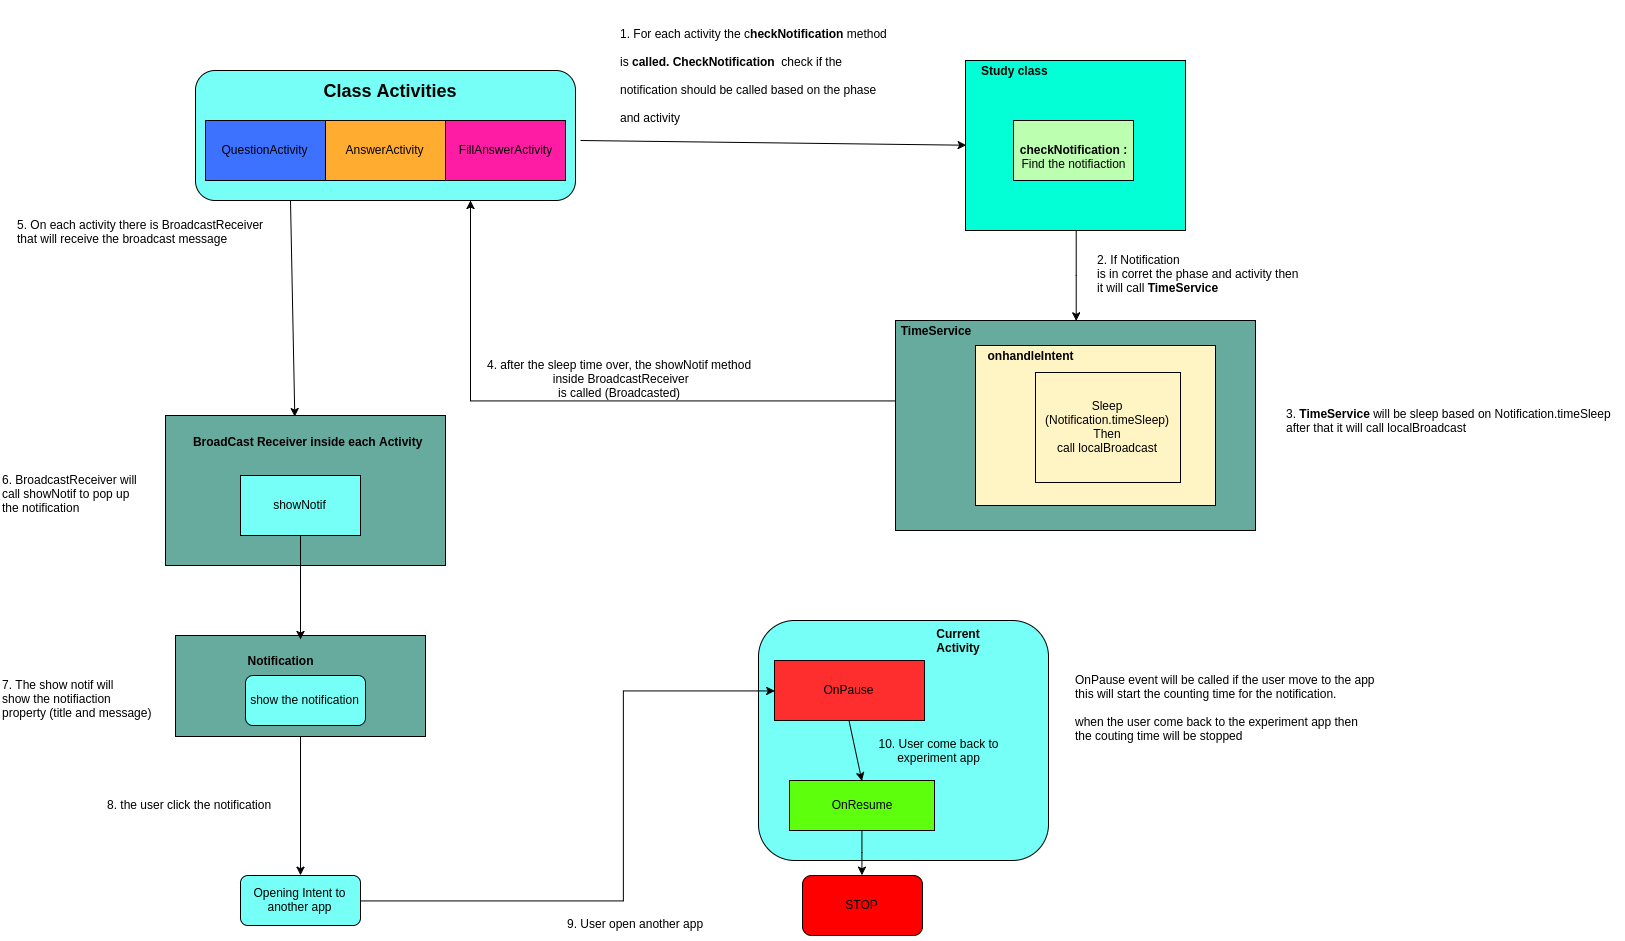
\includegraphics[scale=0.35]{notification_diagram}
\end{center}
\caption{The flow of the notification}
\label{fig:NotificationFlo}
\end{sidewaysfigure}
%
\begin{figure}
\begin{center}
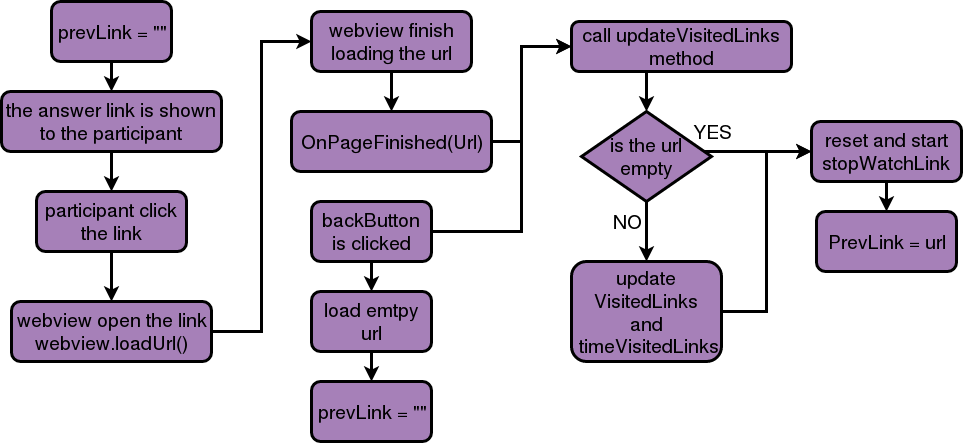
\includegraphics[scale=0.45]{tracker_linkVisited}
\end{center}
\caption{tracker mechanism for webview}
\label{fig:webViewTrack}
\end{figure}

q
\chapter{Experiment Result and Discussion}

This chapter provides the result and the analysis of the experiment. three hypothesis are analyzed;
\begin{itemize}
  \item{Do participant experience the failure of prospective memory while using the smartphone?}
  \item{Is failure of prospective memory is more likely to happen with two intentions rather than one; intentional load matters}
  \item{What is the effect of notification to prospective memory error}
  \item{Does mentaly moving through event boundary increase the likeliness to experience failure of prospective memory?}
\end{itemize}

\section{Prospective memory error on smartphone}

\subsection{Experiment result}
In these expriment the data from the participants from the three studies is combined.
Table \ref{fig:affirmationTable} shows who many participants believe that they have experienced prospective memory error,
and how many participant actually experience the prospective memory error during the experiment.
The participant were asked if they believe that they had experince prospective memory error using the first question on the Table \ref{tab:demographicQuestion}.
Actual experience of memory error was calculated by looking if the people forget the questions during the experiment.

%The prospective memory error on the experiment is presented by the lost of intention during the study.
% The first column shows the affirmation on the prospective memory. the number is obtained by asking the participants \textit{"Often people go into a room to do something.  Though they know they intended to do something, they lose track of what they wanted to do.
% This same sort of thing can happen when using a smart phone, as well.  During the study,
% you may have clicked on a link, gone to the website, and then forgot what you intended to look up.  Did that happen to you at all during this study?"} on the post question phase during the experiment.
% While the second column is obtained by counting how many participant forget the question and chosed to look at the question again (lookback) during an experiment.
% The last column shows the total number of the participant participated on each study.
 %or forget the question during the experiment.

\subsection{Discussion}
% As seen in figure \ref{fig:demo1Study1}, \ref{fig:realdemo1Study1}, \ref{fig:demo1Study2}, \ref{fig:realdemo1Study2}, \ref{fig:demo1Study3}, \ref{fig:realdemo1Study3}, the left
% pie chart shows percentage of participant who think they are experiencing prospective memory error, and on the right side shows the percentage of participant who experience
% the prospective memory failure during the experiment.

Most of the participant did not believe that they have experienced the prospective memory error
. In contrast, the output shows that  almost 70\% of the participant actually experienced the prospective memory error.
We can agrue that the participant made an intention for looking the answer before clicking the answer link, but after reading the answer page
they lost their original intention.
As a result they forget the content of the question, and they experience prospective memory error.
This shows that while using a smartphone a person has a high probability of experiencing prospective memory error.
This experiment support the result of Prof. Richard alan Carlson's experiment.

% \begin{table}[]
% \centering
% \label{my-label}
% \begin{tabu}{|X[3,c]|X[3,c]|X[3,c]|}
% \hline
% \multicolumn{3}{|c|}{Study 1}                                                                             \\ \hline
% Affirmation of prospective memory error & \begin{tabular}[c]{@{}l@{}}Forget the questions \end{tabular} & Total Person \\ \hline
% 0                      & 3                                                                 & 4            \\ \hline
% \multicolumn{3}{|c|}{Study 2}                                                                             \\ \hline
% Affirmation of prospective memory error & Forget the questions  & Total Person \\ \hline
% 5                      & 8                                                                 & 11           \\ \hline
% \multicolumn{3}{|c|}{Study 3}                                                                             \\ \hline
% Affirmation of prospective memory error & Forget the questions                                            & Total Person \\ \hline
% 2                      & 2                                                                 & 3            \\ \hline
% \end{tabu}
% \caption{Participant affirmation and their experiment result on prospective memory error on smartphone}
% \label{fig:affirmationTable}
% \end{table}


\begin{table}[]
\centering
\small
\footnotesize
\begin{tabu}{|X[6,l]|X[2,c]|X[2,c]|X[2,c]|}
\hline
                                                                           & Experiment 1 (n=4) & Experiment 2 (n=11) & Experiment 3 (n=3) \\ \hline
How many participant believe they have experience prospective memory error & 0                  & 5                   & 2                  \\ \hline
How many participant actually experienced prospective memory error          & 3                  & 8                   & 2                  \\ \hline
\end{tabu}
\caption{Number of participant from all the studies who believe they have experince prospective memory error and the actual result of the experiment}
\label{fig:affirmationTable}
\end{table}



\section{The effect of multiple intention}

\subsection{Experiment result}
This section shows the result from the second study. On the second study, one or two question are presented to the participant randomly.
A participant intention is to look for the answer. Thus the number of question presented is the number of intention need to be retained.
Using the result we are trying to see  if increasing the number of intention it will make people more likely to experience failure of prospective memory (is the intentional loads matter ?).
Table \ref{fig:oneTwoQuestionForget} shows the total number of times the participant forget the question on the experiment.
It shows that when the participant presented with two question they are 75\% more probably to forget the
question rather than presented by one question.

Figure \ref{fig:TTFA_oneTwoQues} shows how long in millisecond the participants need to write the answer (TTLFA) of each question if one question and if two questions are presented.
The horizontal axis shows the 11 participant and the vertical axis shows the duration of writing. It shows that 63\% (7 out of 11) have longer time
writing the answer if two questions are presented each time. but the remaining two participant have more or less similar time on writing the answer both on
one or two questions presented.
In general figure \ref{fig:TTLFA_oneTwoQuesGeneral} shows how the average writing time on one or two question for all participant in the second study.
It also shows that if two questions are presented then it will take longer time for the people to recall the answer and write the answer.

Figure \ref{fig:lookingAnswer_oneOrTwo} shows the average time each participant spent on looking for the answer on the answer page. The top plot descibe the average time when
the participant look at the question first time. Surprisingly it shows that almost half of the particpants (4 out of 11) spent significantly longer time to look at the answer for one rather than two questions.
The lower plot shows the time spent looking for the answer after the participant look at the question again (lookback). It shows that most of the participant forget more frequenlty the
question and spent longer time on looking for the answer if two questions are presented at each time.

\subsection{Discussion}

The result of this study shows that the amount of intentional loads are important component on prospective memory. Based on the table \ref{fig:oneTwoQuestionForget}, a person is more probable to experience
prospective memory error if the amount of the intention is higher.

Furthermore, the result on figure \ref{fig:TTFA_oneTwoQues} and figure \ref{fig:TTLFA_oneTwoQuesGeneral} shows that the increasing amount intentional loads also make the person harder to recall the content of the intention. On this analysis,
this intention is different with the first intention which looking for the answer, but the intention
is to answer the question and it's formed after the participant found the answer on the answer page. the recall time is presented as the time participant write the answer.

Based on figure \ref{fig:lookingAnswer_oneOrTwo}, the increasing amount of intention also increase the time the participant spent on looking for the answer.
Moreover, when the failure of prospective memory occurs and the person need to look the question again, the time they spent looking for the answer on the two intentions is higher than one intention.
these result shows that the number of intention decrease their cognitive performance which result on the likeliness of experiencing the failure of prospective memory.
This probably because the increase of intentions will reduce the level of attention given on the task\citep{Reason1984}, and make
the participant take a longer time to find the answer.


% Please add the following required packages to your document preamble:
% \usepackage{multirow}
\begin{table}[!h]
\centering
\begin{tabular}{|l|l|l|}
\hline
\multirow{2}{*}{Participant} & \multicolumn{2}{l|}{How many times the participant forget the question} \\ \cline{2-3}
                             & One question                  & Two question                 \\ \hline
1                            & 0                             & 1                            \\ \hline
2                            & 1                             & 2                            \\ \hline
3                            & 0                             & 2                            \\ \hline
4                            & 1                             & 0                            \\ \hline
5                            & 0                             & 0                            \\ \hline
6                            & 0                             & 0                            \\ \hline
7                            & 1                             & 0                            \\ \hline
8                            & 0                             & 1                            \\ \hline
9                            & 0                             & 0                            \\ \hline
10                           & 0                             & 2                            \\ \hline
11                           & 1                             & 2                            \\ \hline
Sum                          & 4                             & 10                           \\ \hline
\end{tabular}
\caption{The number of question the participants forget}
\label{fig:oneTwoQuestionForget}
\end{table}

% Hampir 75\% dari kelupaan adalah two questions.
%
% then show that TTLFA time they write the answer also longer
% then show that using two question make people look at the answer longer time,
% turns out not. but most of the time participant look again the answer for two question

\begin{figure}[!h]
\centering
\begin{minipage}{.5\textwidth}
  \centering
  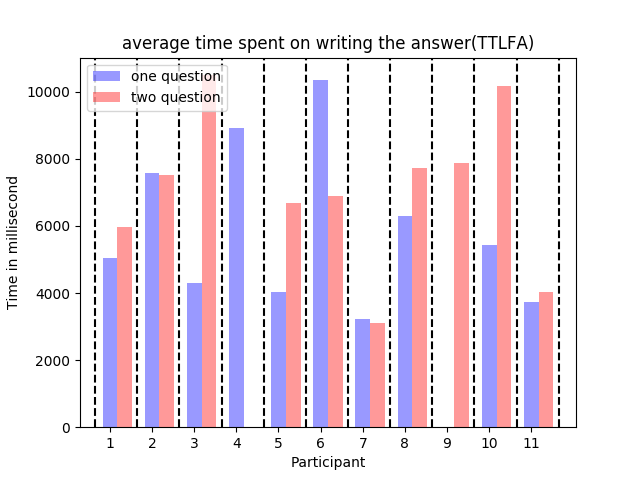
\includegraphics[scale=0.5]{TTFLA_each_participant}
  \captionsetup{justification=centering}
  \captionof{figure}{Average time each participant filling the answer}
  \label{fig:TTFA_oneTwoQues}
\end{minipage}%
\begin{minipage}{.5\textwidth}
  \centering
  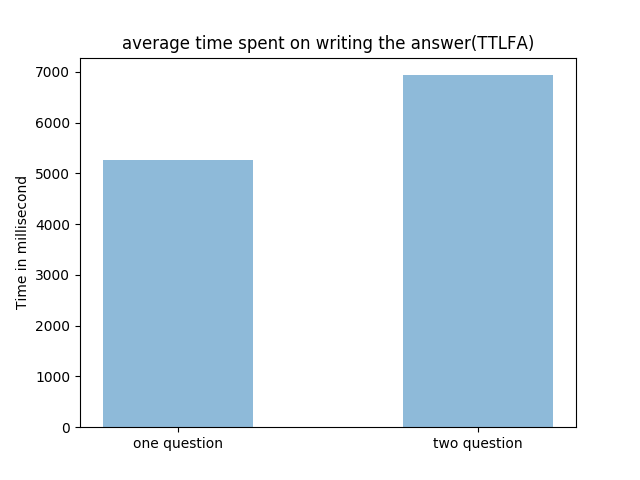
\includegraphics[scale=0.5]{TTLFA_general}
  \captionsetup{justification=centering}
  \captionof{figure}{Average time of all the participants filling the answer}
  \label{fig:TTLFA_oneTwoQuesGeneral}
\end{minipage}
\end{figure}


\begin{figure}[!h]
\begin{center}
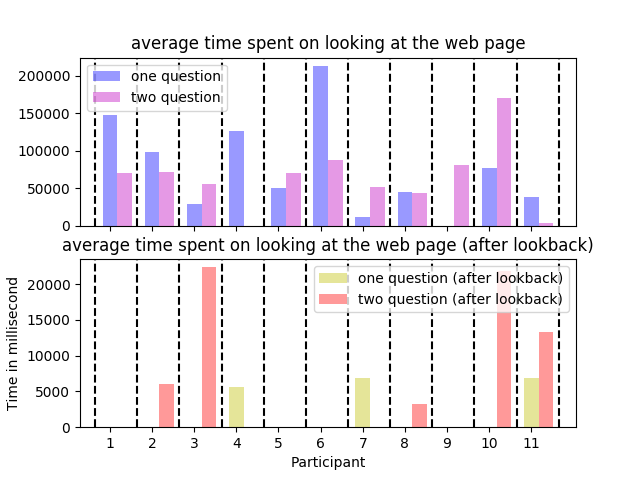
\includegraphics[scale=0.86]{visitedLink_each_participant}
\end{center}
\captionsetup{justification=centering}
\caption{Average time in spent looking for an answer between one or two questions}
\label{fig:lookingAnswer_oneOrTwo}
\end{figure}


% \begin{table}[]
% \centering
% \caption{My caption}
% \label{my-label}
% \begin{tabular}{|l|l|l|l|l|l|l|l}
% \cline{1-7}
% \multirow{2}{*}{Question}           & \multicolumn{2}{l|}{Study 1} & \multicolumn{2}{l|}{Study 2} & \multicolumn{2}{l|}{Study 3} &  \\ \cline{2-7}
%                                     & Yes           & No           & Yes           & No           & Yes           & No           &  \\ \cline{1-7}
% Experience prospective memory error & 0             & 4            & 5             & 6            & 2             & 1            &  \\ \cline{1-7}
% Forget about the answer             & 2             & 2            & 4             & 7            & 0             & 3            &  \\ \cline{1-7}
% \end{tabular}
% \end{table}

% Please add the following required packages to your document preamble:
% \usepackage{multirow}


\subsection{The effect of notifiaction on the intention}
\subsection{Experiment Result}
Table \ref{tab:notifiactionNumber} shows the time participant spent on writing the answer (TTLFA), average time looking for the answer
and the percentage of lookback on each number of notification shown up.
It show that by increasing the number of notification people spent more time writing the answer and looking for the answer.

\begin{table}[]
\centering
\begin{tabular}{|l|l|l|}
\hline
\multicolumn{3}{|c|}{No Notification}                      \\ \hline
TTFA    & Average time looking  at answer page & Lookback percentage \\ \hline
6267.68 & 59875.22 millisecond                   & 17\%                   \\ \hline
\multicolumn{3}{|c|}{One Notifications}                     \\ \hline
TTLFA   & Average time looking at answer page  & Lookback frequency \\ \hline
7292.87 & 69517.0 millisecond                    & 11\%                 \\ \hline
\multicolumn{3}{|c|}{Two Notifications}                      \\ \hline
TTLFA   & Average time looking at answer page  & Lookback frequency \\ \hline
7304.87 & 76699.16  millisecond                   & 21\%                 \\ \hline
\end{tabular}
\caption{The experiment result on each notification number}
\label{tab:notifiactionNumber}
\end{table}

\subsection{Disscussion}
Table \ref{tab:notifiactionNumber} shows that notification and increasing the number of notification make people harder to recall the content of the memory, represented by the average time participant looking for the answer.
We can argue that the notification probably make the level of attention of the participant lower thus make the intention is not framed perfectly
which make the participant experience the detached intention \citep{Reason1984}. Since the notification
also occurs while the participant looking at the answer, interestingly this probably can also mean that the notification distract the intention, even though it's correctly framed before.
Optionaly, the attention probably make the new event model and make people experience new event boundary since the more we present it to the
participant the more they experience harder they recall the content of the intention.

In addition, the notifiaction can also be considered as an event boundary. However, table \ref{tab:notifiactionNumber} shows
that the notification showed up and its quantity is not linear with the percentage of forgetting the question.
So it shows that mentaly moving through event boundary will have no effect on the prospective memory error.

\subsection{Event boundary on prospective memory}
\subsection{Experiment Result}
The bar chart \ref{fig:lookingAnswer_lookback} shows the average time (in millisecond) the participants in all the studies spent looking for the answer on the answer page on each questions.
The chart shows that if the participant forget the question and decide to see it again (lookback), they spent longer time looking for the answer compare to if they don't forget the question(non-lookback).
The bar chart \ref{fig:freq_study1} and \ref{fig:freq_study3} shows the frequency of looking the question again (lookback) for all questions  between first and the third study.
It shows that the peole more frequently do a lookback on third study rathern than on study one.
The bar chart \ref{fig:aveTime_study1} and \ref{fig:aveTime_study3} shows the time spent looking for the answer for all the questions between first and the third study.
It shows that the participant spent longer time to look at the answer and they spent longer time to look at the answer again after the do lookback.
\begin{figure}[!h]
\begin{center}
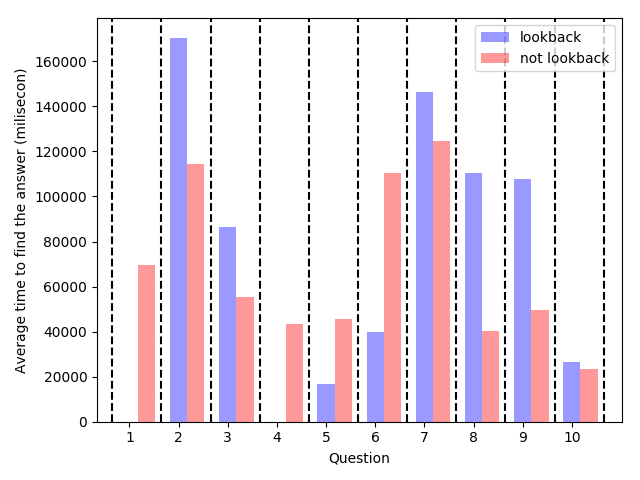
\includegraphics[scale=0.86]{lookback_and_reading_time_studyAll}
\end{center}
\captionsetup{justification=centering}
\caption{Average time in spent looking for an answer between lookback and non-lookback in all studies}
\label{fig:lookingAnswer_lookback}
\end{figure}

\begin{figure}[!h]
\centering
\begin{minipage}{.5\textwidth}
  \centering
  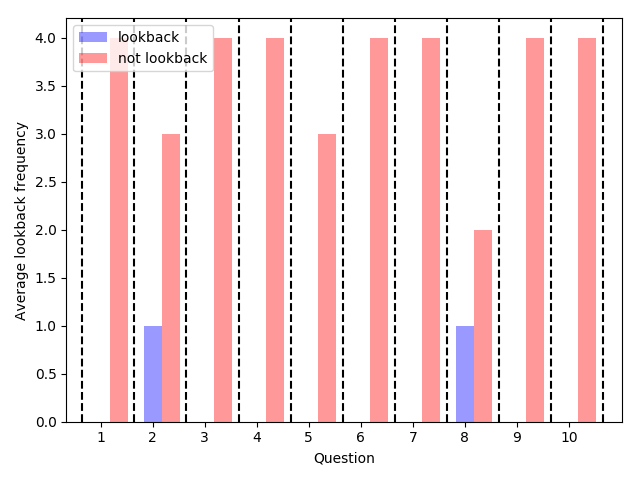
\includegraphics[width=\textwidth]{frequency_lookback_study1}
  \captionsetup{justification=centering}
  \captionof{figure}{Frequency of lookback of the participant on study 1}
  \label{fig:freq_study1}
\end{minipage}%
\begin{minipage}{.5\textwidth}
  \centering
  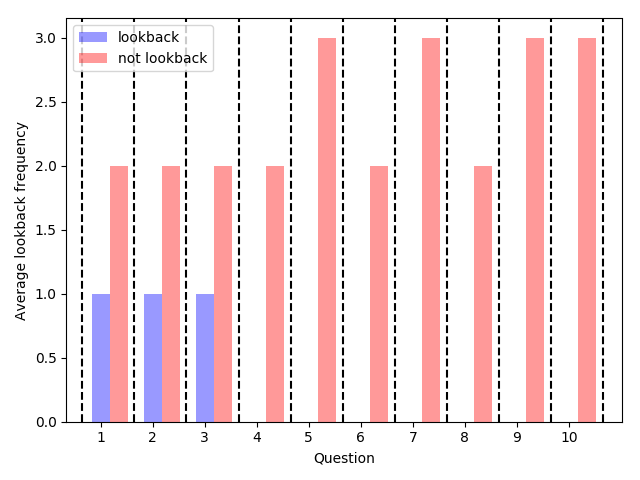
\includegraphics[width=\textwidth]{frequency_lookback_study3}
  \captionsetup{justification=centering}
  \captionof{figure}{Frequency of lookback of the participant on study 3}
  \label{fig:freq_study3}
\end{minipage}
\end{figure}

\begin{figure}[!h]
\centering
\begin{minipage}{.5\textwidth}
  \centering
  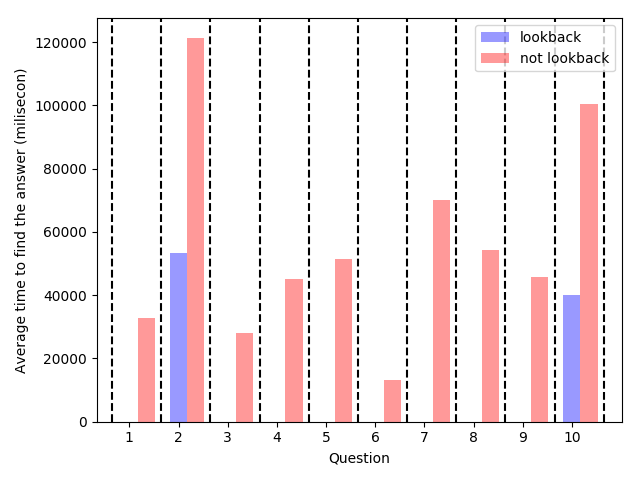
\includegraphics[width=\textwidth]{lookback_and_reading_time_study1}
  \captionsetup{justification=centering}
  \captionof{figure}{Average time each participant looking for the answer in study 1}
  \label{fig:aveTime_study1}
\end{minipage}%
\begin{minipage}{.5\textwidth}
  \centering
  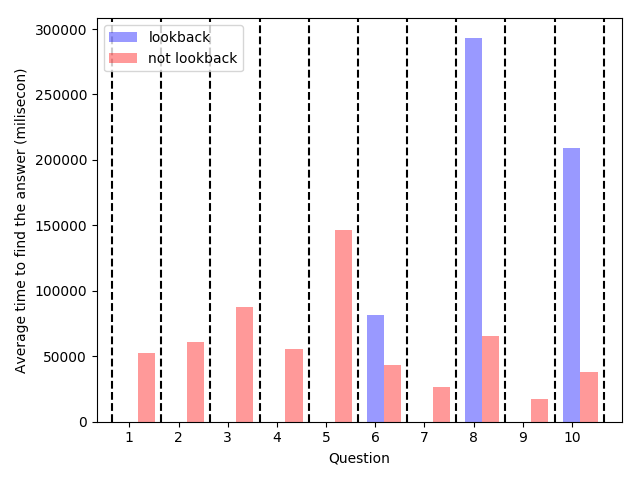
\includegraphics[width=\textwidth]{lookback_and_reading_time_study3}
  \captionsetup{justification=centering}
  \captionof{figure}{Average time of all the participants looking for the answer in study 3}
  \label{fig:aveTime_study3}
\end{minipage}
\end{figure}

\subsection{Discussion}
The result of the bar chart \ref{fig:lookingAnswer_lookback}  shows that the paricipant will more likely to experience prospective memory error if they read longer than the average time
of the participant who do not experience memory error. The participant probably miss the answer or read some interesting information which
make them read longer, then they experience lost intention \cite{Reason1984} as a result they experience  prospective memory error.
We can argue that the participant experience the event boundary which is moving from the android application to the answer page for looking to the answer.
The time spent on reading represent the level of immersion people have on after the event boundary. So the type and the level of immersion of the task after the event
boundary hold a signifact factor on deciding if the person willl experience failure of prospective memory or not.

To understand the effect of physical transition through event boundary we try to investigate the frequency of prospective memory error between first on the third study.
Bar chart \ref{fig:freq_study1} and \ref{fig:freq_study3} shows that the participant on the third study forget the question more frequently than the first study. However,
it cannot show strong correlation between physically moving through another room with prospective memory failure phenomena.
Because the sample is very small so we cannot make any solid conclusions on whether the physical transtition of the event boundary will increase the probability of a person to experience
prospective memory error. However, by looking at bar charts \ref{fig:aveTime_study1} and \ref{fig:aveTime_study3} we can see that the physical transtition result on the longer time for people to read and find the answer.
This shows that the physical transition decrease the capability of cognitive ability while doing this experiment.

\chapter{Conclusion and Suggestion}
\section{Conclusion}
% Chapter 6
% Conclusion
% Valar Morghulis.
% – George R. R. Martin,
% A Song of Ice and Fire


We have successfully build an application that can be used to conduct prospective memory error experiment.
The application support configurable setting which allows researcher to change experiment properties and to conduct
an experiment using a large sample. The application has been made publicly available on the github repository.

By using the aplication three studies has been succesfully conducted.
This study is based on conduct Carlson's studies. From the result of the studies,
we can draw a four conclusion. Firstly, the participant experiences prospective memory error while using the smartphone.
Secondly, the increasing number of intention make people more likely to experience prospective memory error (intentional loads matter).
Thirdly, reducing the number of attention influence the intention but do not increase the probability of prospective memory failure.
Lastly, Moving through event boundary mentally or physically \textit{probably} increase the likeliness of prospective memory failure.
These first two results support the result of Carlson's experiment. While the last one
contradict their result.

% We have presented the
% Track
% application and associated software components as
% a solution to MacLean’s requirement for the development of a custom Android app
% which  would  enable  her  carry  out  an  emotion  management  study  with  adolescents
% at-risk  of  psychosis.   Furthermore,  we  have  implemented  the  application  in  such  a
% way  that  it  can  be  configured  for  use  in  custom  ESM  studies  by  other  psychology
% researchers,  with support for configuration both at the study and survey level.   The
% application also includes an in-app feedback module allowing users to track their emo-
% tions as they progress through the sampling period.
% Track
% has been made publicly
% available on the Google Play store to make it easier for MacLean to distribute to her
% participants, and also supports a non-participant mode for users who want to use the
% app to personally track their daily emotions and activities.
% All  software  components  have  been  made  available  as  part  of  an  open-source
% project on GitHub, and we have also highlighted suggestions for future work which
% can  be  carried  out  to  improve  the  overall  solution.   This  includes  the  implementa-
% tion of a forms-based survey builder to provide a user interface for psychology re-
% searchers to build custom questionnaires with, and extending the current API to enable
% the
% Track
% application to also support a completely configurable feedback module. Once
% MacLean’s study is underway, it would also be interesting to carry out a compliance
% comparison study to determine whether participants making use of the application did
% or did not show a higher compliance rate as compared to others using the paper-based
% version.


\section{Future suggestion}

\subsection{Experiment application suggestion}

To make a more dynamic and ready to public use, the experiment application still have a lot of features that need to be implemented.
The application should have more user friendly setting so the participant can easily set the experiment properties and upload the input file.
On the analysis of the data, it's quite hard to analyze the questions and answer object because there is no field that shows the order of the question, so
it the field that shows the order of the question should be made.

To have better understanding about the event boundary, the question and the answer page presented should be more complex and require
the participant to search the answer by clicking multiple links on the answer page.
Moreover, The application should able to track the movement of the participant so the further analysis can be made on the effect of physical movement
on the failure of prospective memory.


\subsection{Experiment design suggestion}
On the future, I hope that the experiment can be conducted on the bigger sample of participants, and the smartphone of the experiment can be the
personal smartphone of the participant. This will make the participant more comfortable to do the experiment and the failure of prospective memory
phenomena can be analyzed more practically.
I think rather than using a smartphone, the experiment can be conducted by using virtual reality (VR) so the immersion that the participant experience
will be much higher and the study can be more precise on investigating the prospective memory error in everyday life.

\subsection{Futher investigation}
I also suggest that there is a further investigation on the intention and how it stored on the memory. Also, there should be a investigation
whether an intention that is correlated with each other, for example buying a jeans and shirt makes people easier to remember than
buying a cake and a shirt. The motivation to formed the intention should also be investigated, such as giving the participant reward if they do
a better prospective memory task.
% \begin{appendices}
% \chapter{Some Appendix}
% 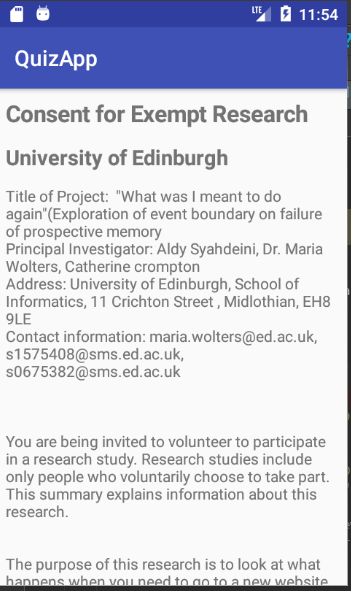
\includegraphics[scale=0.5]{INTRO}
% \end{appendices}


% \begin{figure*}
% \begin{multicols}{3}
% \centering
%     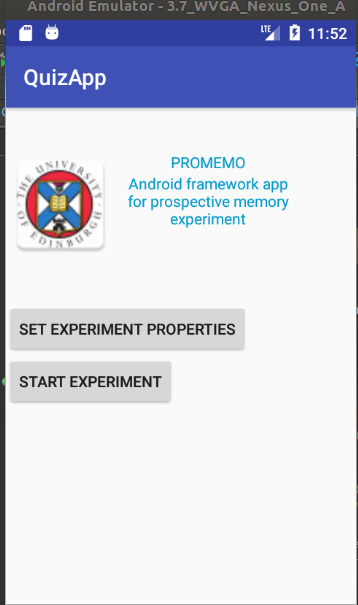
\includegraphics[scale=0.37]{FE_1}
% \caption{}
% \label{fig:ASAs}\par
% 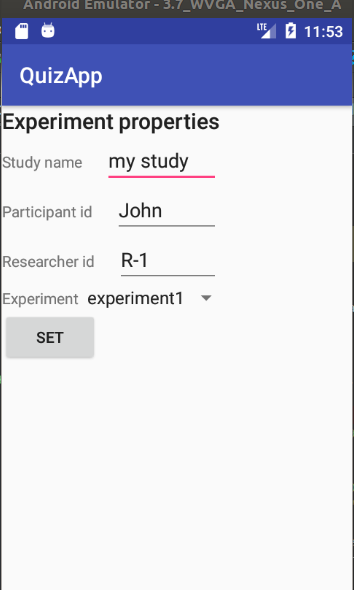
\includegraphics[scale=0.37]{FE_set_properties}
% \caption{Quiz flowchart}
% \label{fig:quiz_flASAsowchart}\par
% 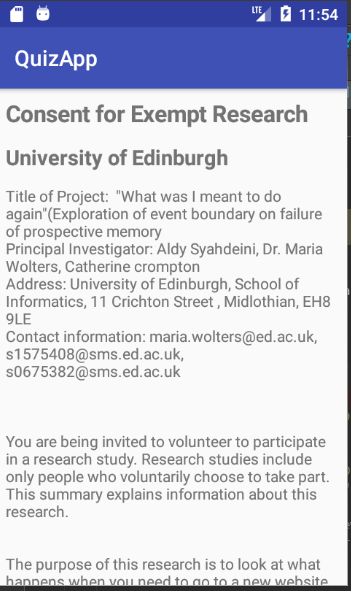
\includegraphics[scale=0.37]{INTRO}
% \caption{Quiz flowchart}
% \label{fig:asdasd}\par
% \centering
%     \end{multicols}
% \end{figure*}


% 
\chapter{Literature Review}
\section{Prospective memory and retrospective memory}

Tasks such as buying milk in a supermarket on the way to work action, turning off the oven and taking a medication are categorized as a prospective memory task. Prospective memory is used constantly in everyday activity \citep{gruneberAndMoris1978}, \citep{cohen1989}.
There are a lot of definition about prospective memory, but generally  a prospective memory is defined as remembering to carry out planned actions at a particular time in the future without being instructed to do so \citep{mcdaniel2007prospective}; \citep{GROOT2002}. While task such as answering the question on an exam or remembering the person name on the party is categorized as a retrospective memory task.
Retrospective memory involves remembering events, words, and so on from the past typically
when deliberating trying to do so.

% The important difference between retrospective and prospective is prospective memory involve remembering to carry out intended actions without being instructed to do so.
% \todo[inline]{keknya paragraph dibawah ini perlu di ubah}


% Remembering in prospective memory is difficult because it require the interuption of flow of thought when we are on ongoing activity, in retrospective memory this interuption is externaly promted e.g question during exam. this made retrospective memory driven by high perceptual information while retrospective  while prospective memory perform on low information content. (McDaniel et al., 1998)

According to \cite{BaddeleyWilkins1983}, it's very hard to differentiate between prospective memory and retrospective memory because there is no clear cut between them, for example, To remember to call your father, you should able to recall his number and how to use the phone, and not call him while he watches a football match. \cite{brandimonte1996prospective} call this as the retrospective component of a prospective memory task.
\cite{CockburnJ.1995Tiip} stated that content of the information is similar to both memory type but the essential difference is prospective memory require memory for intention and the cue for retrieval has to be self-initiated.
\cite{GuynnMelissaJ.1998PMWR} also state that retrospective memory is driven by low information content while retrospective memory is driven by high perceptual information, such as question during an exam.

Furthermore, Remembering only the retrospective memory component of a prospective memory task will not produce successful prospective memory. In fact, numerous prospective memory failures happened because the failure of remembering the prospective memory component
\citep{einsteindGuynn1992}. Interestingly, the component of retrospective memory sometimes forgotten in a simple prospective memory task, for instance when we walk to the kitchen and sometimes forget what we are intended to do there \citep{brandimonte1996prospective}.

% Retrospective memory focus on remembering the content of information like or what we know about something, while the prospective memory focus on implementing the delayed intention or when to do something (Baddeley, 1997).

\section{Cognitive process of prospective memory}
%\todo[inline]{this last paragraph is actually sampah, our focus is what makes us forget not what make us remember}

% This memory division is based on the cognitive processes and Neuroanatomy bases which determine these types of memory . (Maylor, 1995) (Bieriet al., 2014) (Tierney et al., 2016)

Some researcher believes that prospective memory proceeds  through encoding, retention, retrieval, execution and evaluation phase.
According to \cite{inside1996prospective} In the Encoding phase, the \textit{when}(retrieval criterion), \textit{what}(action to be performed) and \textit{that}(intent or decision to act) are encoded. Then this intention representation must be retained until the opportunity to fulfil the intention occurs. This delayed can vary from a second to a week. \cite{EinsteinGillesO.1990NAaP} categorize  retrieval process into two categories;
event-based retrieval and time-based retrieval. On the event based retrieval, the retrieval happens if there is a particular event or physical stimulus that associated with the intention. for example telling a message when you meet your college. On the other hand,
time-based retrieval require execution of action after a certain time  \citep{inside1996prospective};   \citep{Mcgann2002}.
Therefore, successful prospective remembering can be described as a process that supports the actualization of
delayed attention and the associated action,
 and it is strongly associated with control or coordination of future action \citep{inside1996prospective}.

\section{prospective memory error}
% \textit{In this thesis the term "failure of memory error" is also used}.

Prospective memory error is defined as a failure to do a planned action at some point or a particular event in the future.
\cite{Kliegel1984} state that prospective memory failure is the most frequent memory failure in everyday life.
The ability to remember the planned action is a critical factor in human functioning. The consequence of a failure of prospective memory can be trivial, for example forgetting to buy some milk on the way home from work.
But it can also have severe consequences, for example the doctor forget to took the scalpel from his patient after an operation.
In fact, \cite{Shorrock2005} reported that 38\% of accidents on the traffic controllers in the UK was due to memory error involves the failure of prospective memory.

Many researchers have different view on the prospective memory error and what cause it to happen.

\cite{LiaKvavilashviliAndJudiEllis} try to differentiate a various kind of memory error with a prospective memory error. They claim that \textit{action-slip}\citep{HeckhausenHeinz1990IAaA},
 \textit{actions-not-as-planned} \citep{Reason1979-REAANA-2} and \textit{absent-minded error} \citep{cohen2008memory} should not be considered as a prospective memory error. These errors happen because the failure that occurs during the execution or performance of the intended action, for example in absent minded error people lose the context of an intention and carry out an unintended action instead of the intended one. In contrast, prospective memory is focused on the failure to retrieve intended action.
While \cite{10.1371/journal.pone.0074447} argue that these type of error should be considered as part of prospective memory error because prospective memory contains some element of retrospective memory such as the context of intention. Moreover, \cite{Reason1984} explained further on how the element of memory; context, intention and attention influence prospective memory error.  In addition, \cite{Cockburn1994} argued that stress and anxiety make a person to experience absent minded error hence make a
prospective memory error, and \cite{Scullin2012} found older people tend to make more error than younger people on a prospective memory test.

\section{Prospective memory and intention}
Because prospective memory refers to remembering intentions so it would be better to have a good understanding of intention first. For example to understand the nature of intention and its
phenomena, the category of intention and how it related to everyday activities and what happens to intention during prospective memory error. The explanation of these question maybe gives us more understanding about the correlation between intention and prospective memory error.

\cite{LiaKvavilashviliAndJudiEllis}, \cite{gauld1977human} define an intention as a person's readiness to act in a certain way in the future. What has to be done and when to be done should be defined clearly.
\cite{searle1983intentionality} distinguished intention into two types, prior-intention and intention-in-action. A prior intention is an intention that is defined prior to action, while intention-in-action is a spontaneous action, for example going to the toilet when you need to urinate. A prior intention always occurred as a result of conscious decision to act in a certain way \citep{Heckhausen1985-HECFWT}. Furthermore, \cite{gauld1977human} categorized prior intention into two categories, delayed intentions and immediate intention.The delayed intention is a postponed intention that will be executed at some point in the future, and when a person begins to carry out their prior intention immediately after a decision has been made or after they see a particular cue for the intention.


The difficulty of retrieval of the delayed intention make persons miss the prearranged moment or cues, and this makes people fail to remember. Even though people able to retrieve the delayed intention, but when the intention is initiated and transformed into an immediate intention,  people can still lose their intention and prospective memory error occurs.
Furthermore, \cite{Reason1984} explain how a change in the intention make people experience memory error by categorizing two phenomena called \textit{detached intention} and \textit{lost intention}.

\subsubsection{Detached intention}

Detached intention happen if the original content detached from the intention. it will then get replaced or misaplied to another content apart from
its origin.
 For example, the case when a person switches off the television instead of the oven. \citep{Reason1984} explaned that this phenomena happened because the intention is not framed completely.
This premature intention happen probably because a person's attention is focused on other things (this will be explained further on the attention section). Another explanation is the intention
is replaced because it it do not has a sufficient level of retaintion even though the intention is framed completely.
 Another explanation is an existence of intention that has similar content and triger from same object which similar kind of action is appropriate \citep{Reason1984}.


\subsubsection{Lost of intention}

In contrast with detached intentions that happened because of partial failure of the intention and retention system, lost intention
is a complete failure at one or more of the stage of formulation, encoding, storage, or retrieval of the intention.
One typical case is when an intention is lost during the retrieval phase, for instance when a person walks into a room and become aware that he/she can't recall the original intention of the activity \citep{Reason1984}.


\section{Prospective memory and attention}

% Our daily life are strewn with such trifling and usually inconsequential blunders

When we accidentally put our phone in the fridge instead of our food or when we pour the second kettle of water into a freshly made coffee. These slips of action frequently occur as the result of misdirected or diminished attention \cite{Reason1984}
James defines attention as  "the taking possession by the mind, in clear and vivid form, of one out of what seem several simultaneously possible objects or trains of thought".
There is a minimum degree of attentional involvement is necessary to ensure the right execution of the sequence of attentions, and to avoid someone make a mistake due to some kind of attentional failure.

\cite{Reason1984} define attentions as the gatekeeper of consciousness. This definition marks an important role of attention and consciousness in the performance of delayed intention on prospective memory. A person must be conscious of the plan to perform an action. To be conscious about it, the plan should be the focus of attention. The attention should be kept at the encoding phase when the action is planned and at retrieval when the action is performed.

But error can also occur when a person is putting too much attention on the ongoing activity, for example, running down the stair two at a time, this should be an automatic activity but when a person does it with too much attention, then it can be very disruptive.

Moreover, dividing attention is also assumed to reduce the contribution of a controlled process, thereby
reducing performance on a memory test that involves conscious recollection \citep{Jacoby1989}.
Some previous study also shows that there was a substantial reduction in prospective memory performance when attention is divided \citep{McDaniel1998}
\citep{10.1371/journal.pone.0074447}.


\section{Prospective memory error at event Boundaries}

We walk to the park, read a book, watch a movie and do numerous things, one after another. These stream of actions consist of events. How we split up these stream of action into events and stored them into memory influence how we think and what to remember. Memory and cognition are heavily influenced by an event and how a person structures them \citep{Radvansky2012}. \cite{Radvansky2011} introduce an event model which is a mental model that captures the content and structure of an event that people experience.

\cite{Radvansky2012} also suggest that when persons make a cognitive transition from one event to another, they will experience an event boundary. Such transitions can be a change in location, a causal break, the introduction of a new activity, and so on, as long as they involve a shift from one event to another.  On some condition, event boundaries can disrupt memory. When people experience event boundaries, they mentally update their event model. \cite{Radvansky2010} investigate about this phenomena in the reading experiment and shows that the updating effect of a mental model increases the reading time of a sentence.
 The increase of time reflects increase on cognitive effort need for the updating.


% in a series of studies we had done (Radvansky \& Copeland,
% 2006b;  Radvansky,  Krawietz,  \&  Tamplin,  2011;  Radvansky,
% Tamplin, \& Krawietz, 2010)  We  found
% that people took longer and made more errors when there was
% an event shift than when there was not. In other words, walking through doorways caused forgetting.

Furthermore, \cite{Radvansky2010} found that people forget more information if they pass through the doorway to move from
one location to another.
This
effect is similar to the result from other research in text comprehension that shows that shift
in location decline memory performance \citep{Curiel2002}; \citep{Haenggi1995}; \citep{Radvansky2010}; \citep{Radvansky2003}.
Moreover, that study also showed that people were more likely to forget when they passed through two doorways.

\cite{Kurby2008} and \cite{Swallow2009} proposed event segmentation theory
which explains the correlation between memory and event.
 The theory stated that during the experience of an event,
 when event boundaries are identified, people segmented information into separate event models and then stored it into memory.

All these previous research result in event horizon model proposed by \cite{Radvansky2012}
This model also supports an event segmentation theory. The model explained that when an event is
segmented and stored as event model, it declines in availability and become deactivated. And
as person experience event boundaries, a new event model is created in working memory. The
active event model that is currently in the working memory is foregrounded which make it easier
to retrieve, and an available processing capacity is directed to it.

The presentation of a memory cue causes both models that contain target information to
be activated this result on competition and interference, which slows down response times and
increases error rates. This is why returning to a previous room does not improve memory for
objects that were encountered there, and why passing through two doorways makes memory even
worse than does passing through one \citep{Radvansky2011}.


\section{The Experiment}

The experiment on this thesis is based on the experiment conducted by Lisa. M. Stevenson and Richard A. Carlson from Pennsylvania State University conducted an
experiment on the failure of prospective memory.
Each participant answer trivia questions.
 On each question, an embedded link is presented, and the participant was instructed to find the answer on the web page.
 Subsequently, the participant is asked questions to assess their prospective memory.
The experiment conducted three studies, the studies are explained more on section 3.1.1.
Carlson found that a failure of prospective memory happened when a person uses a smartphone.
They found that the amount of intention is an important factor of prospective memory (intentional loads matter).
Also, they found that there is no improvement or decrement on the failure of prospective memory after the transition in locations.

Carlson implemented the experiment by using Qualtrics, a web-based questionnaire administration tool. And the participant
used their smartphone browser to access the website. While we implemented the experiment by using android application.
While Carlson mostly assessed the participant failure of prospective memory by using a question at the end of the experiment. We were also
asked similar questions, but we also track some variables of participant's activity during the experiment.

We track the frequency of the participant when they forgot the question and decided to see it again, this is useful to analyze what factors made the participant experienced
failure of prospective memory. We track how long the participant spent on finding the answer to understand analyze the retention and retrieval of the intention.
We also track how long they spent writing the answer to analyze how they retrieve the content of the intention. All the tracked variables are explained
more detail on section 3.2.6 and the implementation in section 4.4.

Notification were also shown to the participant during the experiment. The aim of the notification
is to lower the level of attention of the participant. The output of the tracked variable and the occurrence of the notification
were analyzed to see the effect of notification on a failure of prospective memory. The design of the notification is explained further in section 3.2.6, and
the notification mechanism in section 4.3.

in Addition, based an idea of \cite{inside1996prospective}, some may argue that the type of intention on the experiment is not delayed intention
thus it cannot be associated with a prospective memory error. But this view is
refuted by \cite{10.1371/journal.pone.0074447}. According to Carlson, there should be a temporal gap
Between forming the intention and the opportunity to carry it out. Typically, of course, part of that interval is filled by some other task.
In the case of the phenomenon we are trying to capture, that other task is simply moving (physically or on the phone/computer) to the setting that allows the intention to be carried out.

%% ... etc ...

%%%%%%%%
%% Any appendices should go here. The appendix files should look just like the
%% chapter files.
\appendix
% \begin{appendices}

\begin{appendices}
\chapter{Study object properties}

\begin{table}[!h]
  \centering
\begin{longtable}{ |p{0.5cm}|>{\hspace{0pt}}p{5.5cm}|p{1.6cm}|p{7cm}|  }
 \hline
 \multicolumn{4}{|c|}{Input} \\
 \hline
 No& Name & Type & Description \\
 \hline
 1 & Study.PreText  & String & Html string that will be shown at first on the experiment\\
 2 & Study.PostText & String & Html string that will be shown after the pretext\\
 3 & Study.Name &  String & The name of the study \\
 4 & Study.Id & String & The Id of the study \\
 5 &  Experiment.Name & String & The name of the experiment \\
 6 & Experiment.NumQuestion & Integer & The amount of questions to be presented on each quiz phase \\
 7 & Experiment.MaxPresentedQuestion  & Integer &  The maximum number of presented question if it change randomly on each phase \\
 8 & Experiment.RandomPresentedQuestion & Boolean &  Whether the number of presented question will be change randomly on each phase \\
9 & Category.Id  & String &  Id of the category \\
10 & Category.Name  & String & The name of the category \\
11 & Category.TotalQuestion & Integer  & The total size of the question on the category  \\
   12 & Category.QuestionOrder  &  String &  The order of how the question will be pulled from the list of questions. "LINEAR" it will be pulled based on the input order, "RANDOM" it will be pulled randomly\\
   13 & Category.Question.Id  &  String & The unique Id of the question \\
   14 & Category.Question.Text  & String &  The question text \\
   15 & Category.Question.linkAnswer  &  String & the URL link of answer \\
   16 & Category.Question.Answer  & String & the answer of the question \\
   \hline
\end{longtable}
 \caption{Explanation of the entities inside the input file}
 \label{tab:inputFile}
\end{table}

\begin{table}[!h]
  \centering
\begin{longtable}{ |p{0.5cm}|>{\hspace{0pt}}p{5.5cm}|p{1.6cm}|p{7cm}|  }
 \hline
 \multicolumn{4}{|c|}{Input} \\
 \hline
 No& Name & Type & Description \\
 \hline
17 & Notification.App  & String & What application the phone will open if the participant click the notification \\
 18 & Notification.shift & Int &
 The number of phase when the notification should be shown. This will be explained more on the Notification section \\
 19 & Notification.Phase  & String & The activies name when the notification should be appeared\\
20 & Notification.TimeToShow & Integer  &  how millisecond the application should wait before showing the notification \\
 21 & Notification.Url  &  String & what url or id the application will open if the participant clicked the notification \\
 22 & Notification.TitleText  & String & The title of the notification \\
 23 & Notification.MsgText  &  String & The text of the notification  \\
 \hline
\end{longtable}
\caption{Explanation of the entities inside the input file}
\label{tab:inputFile2}
\end{table}


\end{appendices}



\begin{appendices}
  \chapter{List of documents used in the experiment}

  \begin{figure}[h]
  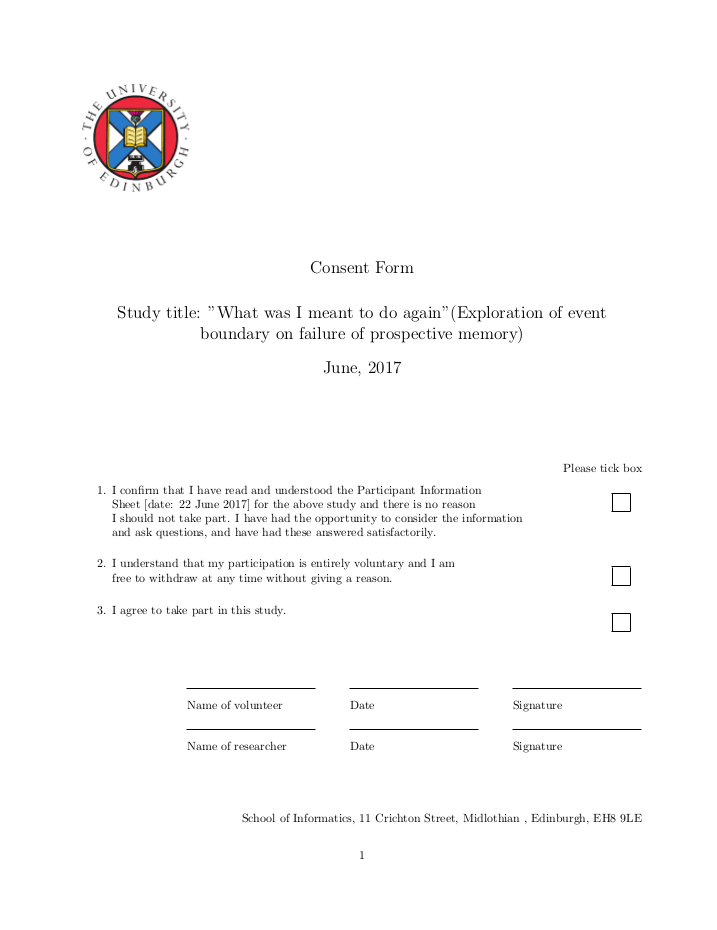
\includegraphics[scale=0.7]{consent_form}
  \caption{Consent form used in the experiment}
  \label{fig:consentForm}
  \end{figure}

  \begin{figure}[h]
  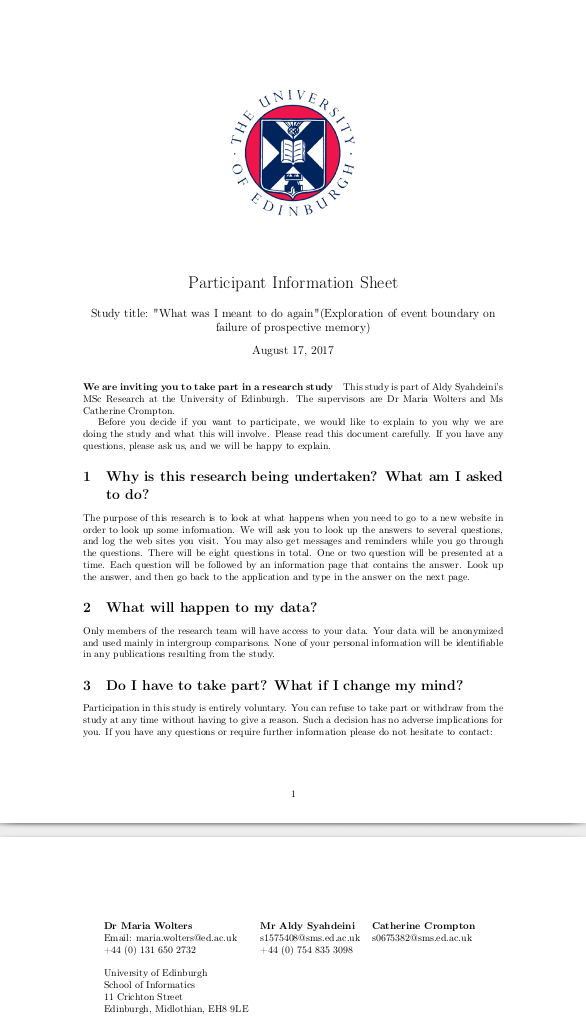
\includegraphics[scale=0.7]{information_sheet}
  \caption{Information sheet used in the experiment}
  \label{fig:InformationSheet}
  \end{figure}

\end{appendices}



  \chapter{Figures of UI layout}

  \begin{figure*}
  \centering
  \begin{minipage}[b]{.4\textwidth}
  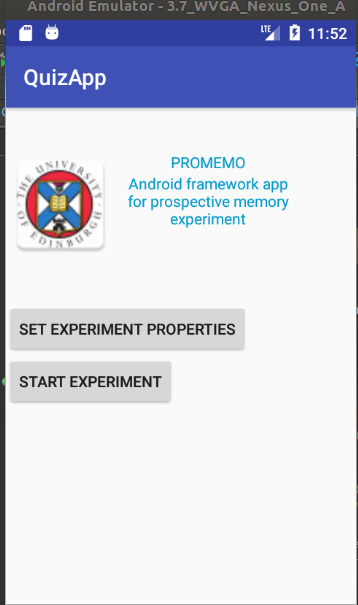
\includegraphics[width=\textwidth]{FE_1}
  \caption{expInitialActivity UI layout}
  \label{fig:expInitialActivity}
  \end{minipage}\qquad
  \begin{minipage}[b]{.4\textwidth}
  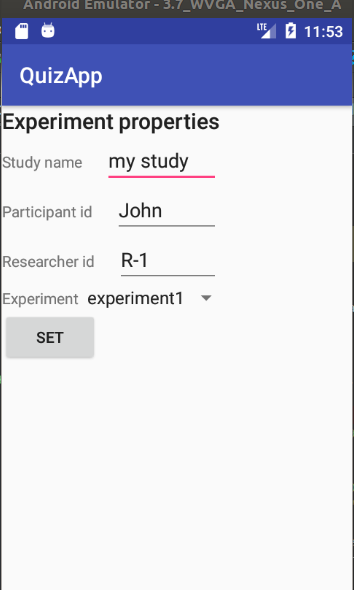
\includegraphics[width=\textwidth]{FE_set_properties}
  \caption{expSetPropActivity UI layout}
  \label{fig:expSetPropActivity}
  \end{minipage}
  \end{figure*}

  \begin{figure*}
  \centering
  \begin{minipage}[b]{.4\textwidth}
    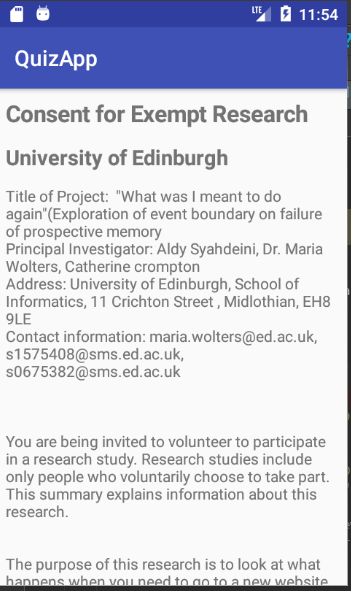
\includegraphics[width=\textwidth]{INTRO}
    \caption{IntroActivity UI layout}
    \label{fig:IntroActivity}
  \end{minipage}\qquad
  \begin{minipage}[b]{.4\textwidth}
    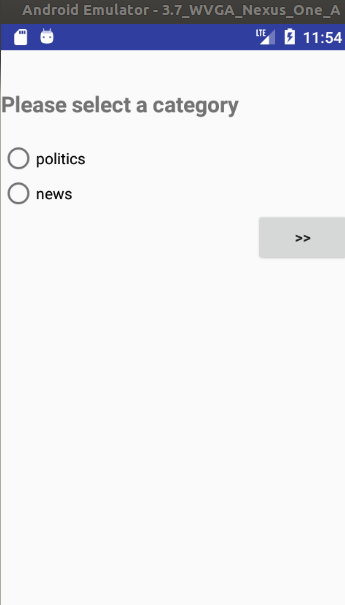
\includegraphics[width=\textwidth]{select_category}
    \caption{ChooseCategoryActivity UI layout}
    \label{fig:ChooseCategoryActivity}
  \end{minipage}
  \end{figure*}

  \begin{figure*}
  \centering
  \begin{minipage}[b]{.4\textwidth}
    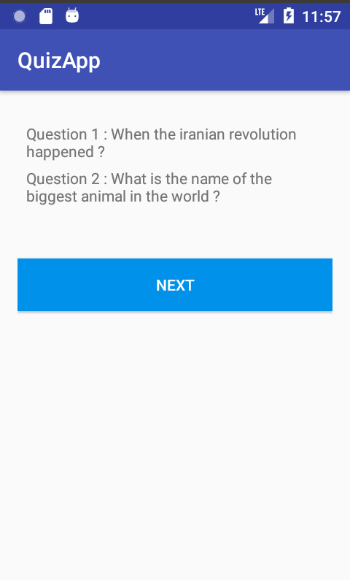
\includegraphics[width=\textwidth]{quiz}
    \caption{QuestionActivity UI layout}
    \label{fig:QuestionActivity}
    \end{minipage}\qquad
    \begin{minipage}[b]{.4\textwidth}
      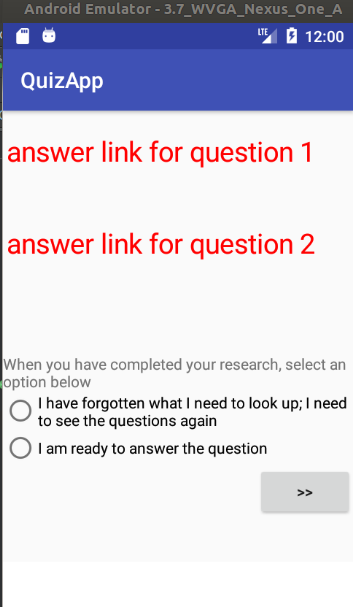
\includegraphics[width=\textwidth]{answer}
      \caption{AnswerActivity UI layout}
      \label{fig:AnswerActivity}
    \end{minipage}
  \end{figure*}

  \begin{figure*}
  \centering
  \begin{minipage}[b]{.4\textwidth}
    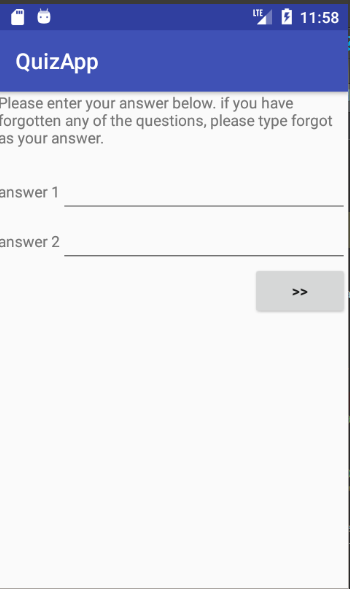
\includegraphics[width=\textwidth]{fillAnswer}
    \caption{fillAnswerActivity UI layout}
    \label{fig:fillAnswerActivity}
  \end{minipage}
  \end{figure*}


  %
  % \begin{figure*}
  % \centering
  % \begin{minipage}[b]{.4\textwidth}
  %   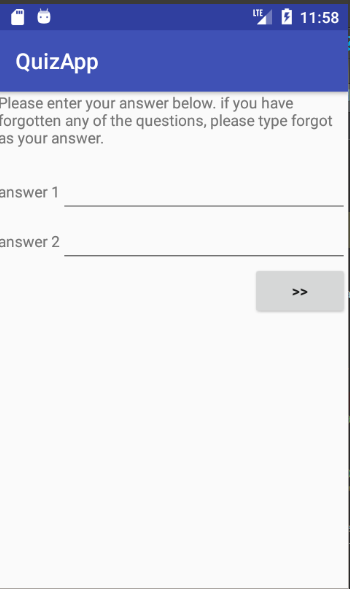
\includegraphics[width=\textwidth]{fillAnswer}
  %   \caption{fillAnswerActivity UI layout}
  %   \label{fig:FE_set_properties}
  % \end{minipage}\qquad
  % % \begin{minipage}[b]{.4\textwidth}
  % %   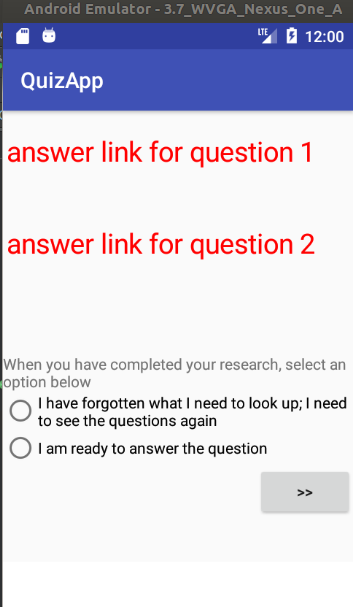
\includegraphics[width=\textwidth]{answer}
  % %   \caption{AnswerActivity UI layout}
  % %   \label{fig:FE_set_properties}
  % % \end{minipage}
  % \end{figure*}

  % \begin{figure}[h]
  % 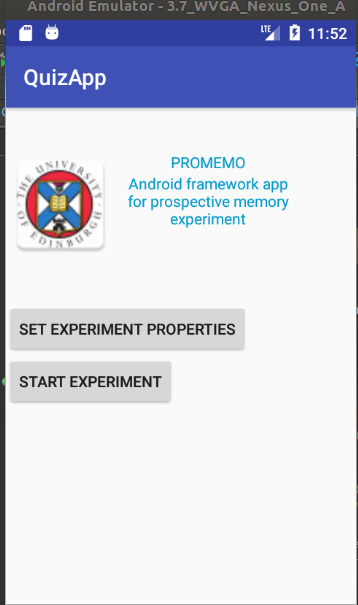
\includegraphics[scale=0.7]{FE_1}
  % \caption{expInitialActivity UI layout}
  % \label{fig:expInitialActivity}
  % \end{figure}

  % \begin{figure}[h]
  % 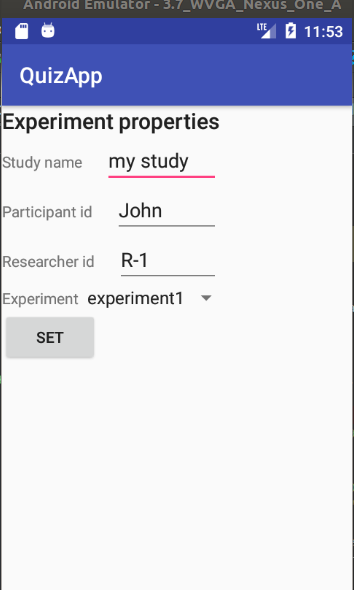
\includegraphics[scale=0.7]{FE_set_properties}
  % \caption{expSetPropActivity UI layout}
  % \label{fig:FE_set_properties}
  % \end{figure}


  % \begin{figure}[h]
  % 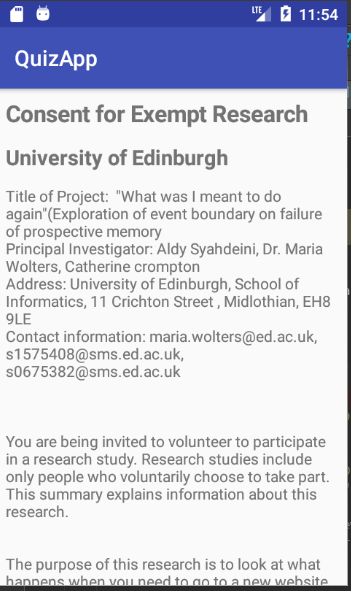
\includegraphics[scale=0.7]{INTRO}
  % \caption{IntroActivity UI layout}
  % \label{fig:FE_set_properties}
  % \end{figure}


  % \begin{figure}[h]
  % 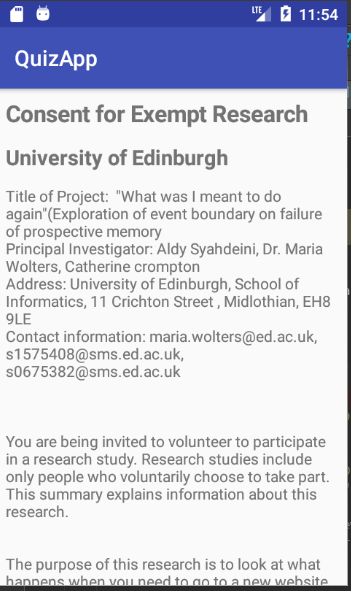
\includegraphics[scale=0.7]{INTRO}
  % \caption{IntroActivity UI layout}
  % \label{fig:FE_set_properties}
  % \end{figure}


  % \begin{figure}[h]
  % 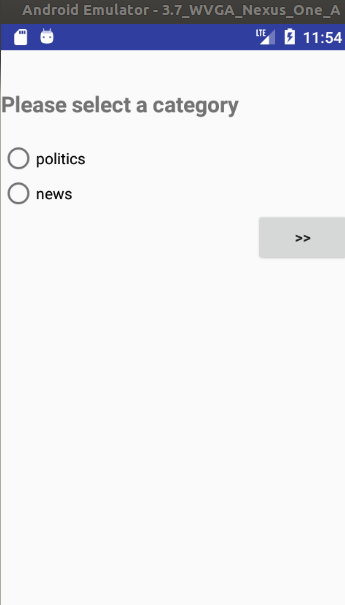
\includegraphics[scale=0.7]{select_category}
  % \caption{ChooseCategoryActivity UI layout}
  % \label{fig:FE_set_properties}
  % \end{figure}


  % \begin{figure}[h]
  % 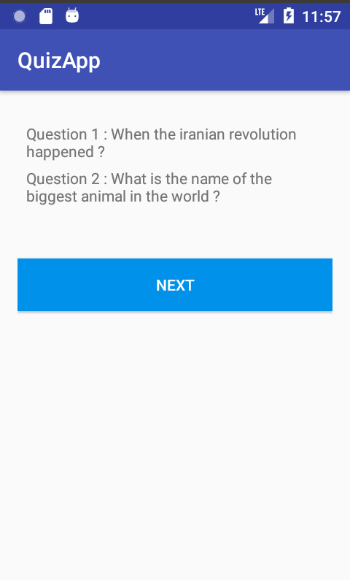
\includegraphics[scale=0.7]{quiz}
  % \caption{QuestionActivity UI layout}
  % \label{fig:FE_set_properties}
  % \end{figure}

  % \begin{figure}[h]
  % 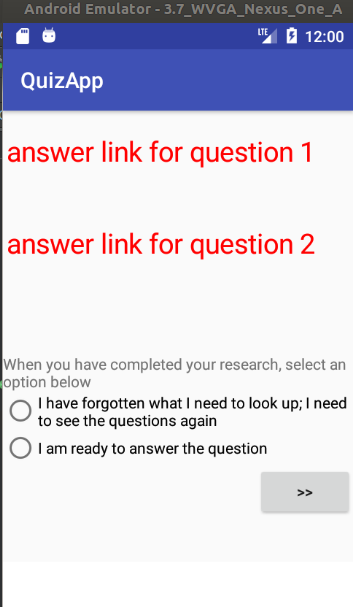
\includegraphics[scale=0.7]{answer}
  % \caption{AnswerActivity UI layout}
  % \label{fig:FE_set_properties}
  % \end{figure}

  % \begin{figure}[h]
  % 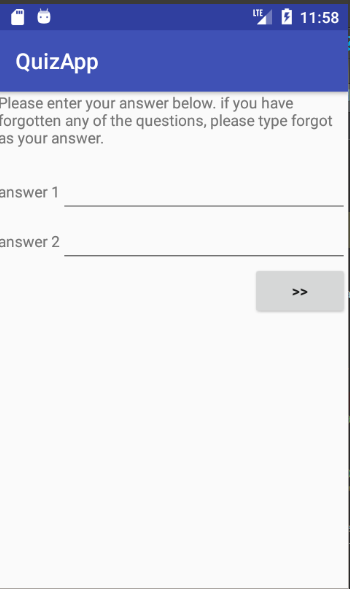
\includegraphics[scale=0.7]{fillAnswer}
  % \caption{fillAnswerActivity UI layout}
  % \label{fig:FE_set_properties}
  % \end{figure}

%% ... etc...

%% Choose your favourite bibliography style here.
%% If you want the bibliography single-spaced (which is allowed), uncomment
%% the next line.
% \singlespace

%% Specify the bibliography file. Default is thesis.bib.

\bibliographystyle{apalike}

\bibliography{resources/myref}


%% ... that's all, folks!
\end{document}
